\selectlanguage{english}

\chapter{Computer-assisted language learning}
\label{ch:call}

%
% 
% this chapter, we will talk about computer assisted language learning, this is for L2 learning.

% add in - BirdBrain, predict probability of getting an exercise right, use that to give you exercises in your zone of proximal development
% AI tools help to decide the levels of sentences and vocab to sequence it correctly although people write it
% they use the idea of zone of proximal development
% a/b testing -- keep some people the same, try a new feature with other people, see if it has an effect, like an experiment, cool, talk about this too, compare learning outcomes.
% content length - how long are the sentences that you can translate accurately?
% time spent learning 

\section{Introduction}

At the intersection of language and educational technology, the field
of \keyword{computer-assisted language learning (CALL)} develops tools
that help you learn a second language.  In this chapter, we explore how people learn
languages, how digital tools can support them, and what such tools
need to know about language.

\section{Learning language}

You already picked up your first language (\keyword{L1}) as a baby.
Later on, you probably encountered a second language (\keyword{L2}) in
a classroom or when you visited another country.  When we speak here
of first and second language, we should not take this literally. If
you grew up bilingually, in a context where multiple languages were
spoken, you can have more than one L1; and L2 typically is used to
refer to all languages that you learned after your L1
was in place, even if this actually was the third or fourth language
you learned.

This chapter focuses on computer-assisted tools for learning an L2,
but it is informative to first compare and contrast how people learn an L1 versus an L2 in general.

\subsection{Similarities between L1 and L2 learning}

Learning any language involves many different aspects. You have to
learn how to articulate the sounds with your mouth
(\keyword{articulatory phonetics}), or, for signed languages, how to
form the signs with your body; how sounds can combine
(\keyword{phonology}), how to form words (\keyword{morphology}) and
sentences (\keyword{syntax}), and what they mean
(\keyword{semantics}).  You might not be able to state these rules explicitly unless you have training in linguistics, but you know them implicitly as
part of your ability to speak a language.

You also have to learn a lot of \keyword{vocabulary} -- thousands of
sound/meaning pairs, memorized so well that it feels subconscious --
as well as statistics about what words are likely to appear in
sequence in which context.  You have to learn social skills such as
how to have a conversation, how to model someone else's beliefs and
goals, and what you should say in different situations (competence in
\keyword{turn-taking}, \keyword{pragmatics}, and \keyword{discourse}).
And you have to learn about the culture of the people you talk to in
this language -- the history, politicians, holidays, music, etiquette,
and foods that people take for granted (\keyword{cultural
competence}).  Moreover, to function in a literate society, you have
to learn to read and write, and how to write for different purposes, in
different genres.

Whether you are learning an L1 or an L2, there are some similarities.
Comprehension precedes production: At each stage of learning, you can
understand more complicated vocabulary and sentences than you can
produce yourself.  Simple sentences are learned before complex
sentences, and frequent words are (mostly) learned before infrequent
ones.  People learning their L1 or their L2 also make similar types of
``errors'', saying things that a full-grown L1 speaker would not say.
To use an example from articulatory phonetics, when learning English
as an L1 or an L2, people struggle to pronounce the [\dh] fricative in
the word \exword{the} -- sometimes pronouncing it as the
stop [d], which shares the same general tongue placement and
voicing. Interestingly, most languages do not use the sound [\dh] in
their system of phonemes -- and, indeed, it is often the case that the
harder something is to learn, the more rare it is across different languages.  As
for grammatical errors, both L1 and L2 learners of English may
\keyword{over-regularize}, for example applying the rule for marking
past tense even on irregular verbs (e.g., producing \exword{*I goed}).

Turning to vocabulary, both L1 and L2 learners may make errors
involving \keyword{over-extension} of word meanings, for example
using the word \exword{car} to describe trucks or golf carts.  They
might also struggle with \keyword{under-extension}, for example, using
\exword{car} for road vehicles while not realizing this word can also
apply to the chunks of a train.  Of course, under-extension may not
give rise to obvious errors the way over-extension can, which points
to a deeper methodological question in the study of language learning:
even if a language learner appears to understand a word or to use it
sensibly, how do you know if they understand it the same way as
another speaker?

\subsection{Unique elements of L1 learning}

Even though L1 and L2 learning involve similar steps and error
patterns, there are also many differences between acquiring an L1 and
learning an L2 in different contexts.  For their L1, a child
understands and produces speech (or signs) long before they learn to
read and write.  The child has to pick up a lot of non-linguistic
information at the same time: They have to develop concepts of
themselves, other people, and of physical and mental events and
entities.  

As their first steps towards vocalizing and communicating, babies can
 cry at birth and smile at around six weeks.  They explore more
 complex vocalizations soon after, and by about six months, babies
 typically begin using sequences of consonants and vowels such as
 \exword{bababa}, a stage referred to as \keyword{babbling}. Next,
 their first words tend to be names for people and physical objects
 (\exword{Dada, doggie}), with other words -- abstract nouns such as
 \exword{happiness}, verbs such as \exword{walk}, grammatical markers
 such as \exword{the} -- coming later on.  Children quickly start
 learning words by their first birthday and can form simple two-word
 utterances by the time they turn two.  Children then make use of more
 and more of the language structure, so that by the age of three they
 can already voice and understand sentences of surprising
 complexity. In the following years of childhood, more and more words
 and complex language structures are acquired, with some structures
 such as passive sentences being added relatively late, around nine or
 ten years of age.  When learning their L1, the child has no other
 language experience to \keyword{transfer}, neither to help them nor
 to confuse them.



Children learn their L1 from the \keyword{input}  provided by their caregivers, which takes the form of \keyword{child-directed speech}.  Across many different cultures, adults speak differently to children than to other adults: They use simple words, repetitive sentences, and highly variable pitch to capture the child's attention; they narrate daily activities, point at objects to name them, and rephrase the child's utterances in more adult terms. 

Children all start learning their L1 in infancy.  There are a few extremely tragic cases where children were not exposed to any L1 until later in life and seemed to struggle to learn it.  These situations are confounded by other traumatic elements, so it is hard to draw clear conclusions and unethical to run studies, but they are sometimes taken as evidence that L1 learning must occur in a \keyword{critical period} of a child's life, before adolescence, to be fully successful.


A child learning their L1 gets quite a few hours of input and practice each day, and -- even if they can't reflect on it -- has an extremely strong incentive to succeed, because they need to learn language to participate in society. As a result, excluding cases of extremely serious  disabilities, all children achieve ``success'' at learning their L1 (at least in speaking and listening, if not reading and writing), in the sense that they all become L1 speakers of it and can use it to say anything they want. 



Although children have a strong incentive to learn their L1 and get lots of practice, they do not receive much formal instruction. All children achieve essentially the same level of ``success'' in learning their L1 even when the input that they receive varies widely across families and cultures.   In this sense (as proposed by \citealt{Lenneberg:67}), learning an L1 is like learning to walk rather than learning to play the piano or dance ballet: All children learn language just like all children (with working legs) learn to walk, regardless of how explicitly their family tries to teach them, whereas children only learn to play the piano through dedicated instruction.  Like walking, therefore, L1 success is sometimes analyzed as an \keyword{innate} human capacity rather than one that \keyword{emerges} from one's experience. That is why it is sometimes referred to as \keyword{L1 acquisition} rather than \keyword{L1 learning}, based on the idea that acquisition is innate and automatic while learning requires explicit instruction.   But the idea of innateness is controversial, since it ties into a huge debate (pervasive across social sciences) about \keyword{nature versus nurture}.
If children are said to be born with certain  knowledge that helps them acquire language, it is very difficult and contentious to spell out exactly what that knowledge would be, and how it complements the input  that they experience.  Whether it is true or not,  the idea of innateness  is inspired by the striking fact that children all learn their L1 successfully and essentially automatically.



\subsection{Unique elements of L2 learning} \label{sec:l2}

Whereas everyone learns their L1 as a child from their caregivers, people learn L2s in different contexts, for example in a classroom or upon immigrating to a new place.  When learning an L2, a person may learn to read and write at the same time as they learn to speak and understand.  The L2 learner already knows quite a lot of general information (how the world works, how conversations work, the idea that words refer to things) which is not obvious to a child learning an L1. And while everyone learns their L1 as a child, people encounter L2s at all ages after they've learned their L1.

Like L1 learners, L2 learners go through different stages and levels of sophistication, but they can learn verbs, abstract nouns, and grammar from day one, depending on the input that they receive.  While a child's first words might be \exword{Dada} and \exword{doggie}, an L2 learner might start with \exword{hello} and \exword{my name is}.


Whereas children learn their L1 from the spoken input of caregivers, people learn their L2 from all sorts of input -- conversations, media, signage, and educational resources.  The L2 learner may also transfer some knowledge of their L1 to their L2, which can both help and hurt them.  L1-to-L2 transfer is useful in the case of \keyword{cognates}, which are words that are similar in both languages (due to a common historical origin or borrowing from the same source); for example,   `coffee' is  \exword{k\={a}f\={e}i} in Mandarin and \exword{caf\'e} in French.  L1-to-L2 transfer can also help with some grammatical rules: If your L1 is English and you are learning French or Chinese, you can carry over the Subject-Verb-Object rule of word order.  
But L1-to-L2 transfer can also cause errors if you transfer something that is not shared between the L1 and the L2, for example incorrectly transferring the Subject-Verb-Object word order to Irish, where the verb comes first. 

A person learning an L2 in a classroom might get about five hours of practice per week, and their incentive is most likely determined by their commitment to the class.  A person learning an L2 as an immigrant will get more or less practice depending on their job and social network, and their incentive may derive from how much they need the L2 to function.  Because the incentives and the amount of practice vary so widely across L2 learners, it is perhaps no surprise that people  achieve wildly different levels of ``success''.  Some people teach classes and write award-winning books in their L2, while other people can barely check in to a hotel after years of schooling.

\subsection{Defining and achieving L2 success}

What does it  mean to succeed at learning an L2?  Ultimately, success is defined by your own priorities.  It could mean that you can function professionally and socially in the L2, that you can produce the L2 without  ``errors'',  or that you can translate  accurately in both directions.  (Which of these would you consider most important?)  Most people would not say that L2 success requires the learner's speech to be completely indistinguishable from that of an L1 speaker; even highly proficient learners may still have an accent influenced by their L1.
 

Various language-teaching organizations have  put forward scales of L2 success.
The American Council on the Teaching of Foreign Languages (ACTFL) ranks speakers as Novice, Intermediate, Advanced, Superior,  or Distinguished (with some levels further subdivided into Low, Mid, and High).  According to the 2024 ACTFL guidelines (with example interview videos at each level on their website), speakers at the  Novice level ``can express basic personal information and satisfy a limited number of
personal needs using formulaic and rote utterances, lists, and phrases'' \citep{ACTFL}.  Their ``limited language control may require a sympathetic
audience to be understood''.  At the other end of the spectrum,  speakers at the Distinguished level ``can negotiate, use persuasive and hypothetical discourse, comment thoughtfully on a range of general topics, and tailor language to a variety of audiences''.

Similarly, the Common European Framework of Reference for Languages (CEFR; \citealt{CEFR}) uses three levels (A=Basic, B=Independent, C=Proficient), each subdivided into a higher and lower portion (A1, A2, B1, B2, and so on).  The lowest level A1 ``can introduce him/herself and others and can ask and answer questions about personal details such as where he/she lives, people he/she knows and things he/she has''\footnote{\url{https://www.coe.int/en/web/common-european-framework-reference-languages/table-1-cefr-3.3-common-reference-levels-global-scale}, accessed 2024-07-01.}. The highest level C2 ``can understand with ease virtually everything heard or read [and] can summarise information from different spoken and written sources, reconstructing arguments and accounts in a coherent presentation''.

These functional \keyword{can-do statements} are designed to capture
the vastly different levels language learners have in making use of a
foreign language. Among Anglophone American high schoolers, even
students who get the top score (5/5) on an Advanced Placement foreign
language exam only get to about an Advanced Low ACTFL level (``able to
participate in most informal and some formal conversations on topics
related to school, home, and leisure activities [\ldots] can also
speak about some topics related to employment, current events, and
matters of public and community interest'').  Among other Anglophones
who don't get a 5 on the exam, the level of
proficiency is lower.  After high school, a student's L2 level may
decline sharply when they stop taking classes; only a few dedicated
Anglophone L2 learners will go on to the Superior/Distinguished levels
by seeking opportunities to practice the language beyond the
classroom.  But across the globe, it is very common for L2 learners to
achieve ``Distinguished'' proficiency in a language that they learn
through immigration or in school to use as a \keyword{lingua franca}
(a language of commerce or higher learning).

Given that different people achieve such different levels of success,
what factors contribute to it?  The researcher Stephen Krashen
\citep{Krashen:1982} argues that an L2 learner achieves greater
success when they receive more ``comprehensible input'' at the
\exword{i}+1 level, meaning input that goes just a bit beyond
(+1) their current level of understanding (\exword{i}).  
This idea echoes the \keyword{zone of proximal development}, an idea from the Soviet psychologist Lev \citet{Vygotsky:1978} used in education theory.
The idea is
that the \exword{i}+1-level input provides a built-in review of what
the learner already knows while also exposing them to new words and
structures that they can figure out from what they already understand.
This theory is meant to explain, for example, why a person who already
took two years of Spanish might improve greatly after a summer in
Mexico, because they receive a lot of language exposure at their
intermediate \exword{i+1} level from commercial transactions,
friendships, and so on.  In contrast, a person with no Spanish
experience might not learn much, because most of this Spanish exposure
lies far beyond their basic \exword{i}+1 level and thus goes over
their head.  Krashen's theory therefore predicts that a classroom
environment is especially important for the early stages of learning,
because it is one of the only places where a student will encounter
input tailored to their low \exword{i}+1 level.  While Krashen's
theory has been critiqued for focusing on comprehension rather than
production, it is certainly the case that students learn best (in all
areas) when they encounter surmountable challenges in their zone of
proximal development.

Another important factor is the learner's attitude.  L2 learners
achieve greater success when they are more motivated; when they have a
positive attitude towards the L2 and its culture; and when they are
willing to make mistakes, using a \keyword{growth mindset} (the belief
that one's mind is a muscle strengthened by exercise, an idea proposed
by the psychologist Carol Dweck and colleagues;
\citealt{BlackwellDweck-etal:2007}).  Of course, these attitudes are
all intertwined, not just with each other but with the amount of input
at the \exword{i}+1 level that the learner will seek out, as well as
their incentive for learning the L2.

The effect of the learner's age remains controversial.  On the one
hand, one might think that it would help to learn an L2 as a child
during the pre-adolescent ``critical period'', the way people learn
their L1, and the fact that adult L2 learners usually retain a foreign
accent suggests that there may be a critical period for articulatory
phonetics.  On the other hand, mature learners have better study
skills, and people can learn grammar and vocabulary at all ages.  In
any case, the effect of age is hard to isolate from all the other
factors that correlate with it, such as the amount of practice the
learner receives and their incentive for learning the language.

Researchers in L2 teaching evaluate various teaching techniques by exploring the
extent to which they advance L2 success by providing more \exword{i}+1
input and/or by sparking the learner's motivation.    Such techniques include tools in computer-assisted language learning. 

\section{Why does CALL need to be ``intelligent''?}

In a broad sense, CALL encompasses all the ways in which computers pervade education and society.  As a general medium for information, computers are used by L2 learners to find and present information -- as a multimedia textbook, a dictionary, a tool for writing and consuming media
content, and a way to connect socially with speakers of the L2.  

More narrowly, CALL describes tools used to present sequenced exercises for language learners, along with feedback on the learner's responses.  The task of CALL is to design these exercises and feedback in the most efficient and helpful ways.

At a simple rote level, one could design a CALL system consisting of dozens of handwritten \keyword{fill-in-the-blank} questions (also known as \keyword{cloze} or \keyword{gap-fill} exercises), which ask whether the learner understands a sentence well enough to complete it sensibly.  If these questions have multiple-choice answers as in \REF{multichoice}, it might take work for the CALL designer to write the \keyword{distractors} (the wrong answers) as well as the correct answer (\exword{on}), but at least it is easy for the CALL system to grade the correct response from among these constrained options.  Alternatively, if the question offers a free-text box \REF{freetext}, then the CALL designer has even more work to do: Instead of writing three distractors, they have to write a longer list of potential right answers -- \exword{on, near, by} and so on -- to assess the learner's answer.

\ea \label{multichoice} The detective lives \uline{\hspace{2cm}} Baker Street.
    \ea at
    \ex on
    \ex in
    \ex with
    \z 

\ex \label{freetext} The detective lives \uline{\hspace{2cm}} Baker Street.
\z 

In a \keyword{frame-based CALL system}, a student's answers are matched against a set of correct and incorrect answers which are explicitly specified by an instructor in a so-called frame such as \REF{multichoice}--\REF{freetext}.  In addition to judging the answer as correct or incorrect, the frame can be designed to include more elaborate pre-written feedback for each of the choices, also known as \keyword{canned text}.  If the learner incorrectly chooses \exsent{in} for \REF{multichoice}, one could specify the feedback \exsent{Incorrect: While the preposition ``in'' can be used for cities, it cannot be used for streets as in this example.}  The system might also need a \keyword{fallback case} if it receives totally unexpected input: If the user types \exword{Help!} in \REF{freetext}, the system could reply: \exsent{You entered Help!, which is not a preposition of English. Please enter a preposition of English.}

The person designing these exercises will use their own metalinguistic insights to organize the exercises at escalating levels of difficulty, for example placing simple sentences (\exsent{The girl eats the apple}) before complex ones (\exsent{The boss didn't realize that the employees were unhappy}) and choosing plausible distractors of the same lexical category as the target answer (as in \REF{multichoice}, where all the choices are prepositions).  They will also use their knowledge of language to write metalinguistic feedback as canned text.  But so far, the simple frame-based CALL system that we have described does not itself distill any insights about language.  As a result, such a system is very brittle and laborious.  Without any deeper representation of language, it just matches
the characters entered by the learner against strings stored as potential answers for the exercise.  If the response matches an expected answer, whether right or wrong, the system can trot out the prescribed action. But if the response is unexpected, the system will have to fall back on default responses, which are unlikely to be very helpful.  This simple system also does not represent any information about the learner; it would just give all learners the same exercises in the same order, which different people might find too easy or too difficult.

In contrast to this hypothetical rote system, modern CALL tools aim to be ``intelligent'' in that they represent information about both the structure of the specific language and the progress of the specific learner.  That way, they can be designed efficiently to offer more exercises, handle more diverse input, and give more helpful feedback that extends even to new or unexpected input.  Such systems also aim to customize the exercises and feedback for each specific learner, so that it's neither too difficult nor too easy.  Next, we will explore how intelligent CALL systems represent both language and learners.



% frame-based versus intelligent CALL tools?




\section{Modeling language}

Now that we have seen why it is useful to capture generalizations about language instead of hand-specifying answers for individual questions, we explore what is involved in realizing this idea.  The application of CALL takes us on a tour of many different tasks involved in text processing more generally. 

\subsection{Parts of speech}

For starters, the words of the target L2 can be automatically labeled for their part of speech (noun, verb, adjective, preposition, and so on), and such labels can be used to give metalinguistic feedback that can be generalized across many exercises. 
 
In English, the transitive verb \exword{buy} requires a direct object (\exsent{I bought groceries}) while the intransitive verb \exword{shop} cannot take a direct object (\exsent{I shopped}).  If the intelligent CALL system represents the allowable \keyword{argument structures} (subject/object configurations) for each verb, then if the learner chooses \exword{shop} in question \REF{shop}, the system could reply: \exsent{``Shop'' is an intransitive verb, so it cannot combine with an object. Please try again.} 

\ea  Maya went to the store to \uline{\hspace{2cm}} flowers for Juan.
    \ea \label{shop}   Fill in the blank: \exword{Buy, shop}.
    \ex \label{whoshop}  Who is going shopping?: \exword{Maya, Juan}.
\z 
\z 

In English, some verbs work like \exword{shop} in that they cannot have a direct object; others work like \exword{buy} in that they need one; while others work like \exword{eat} in that they can go either way: \exsent{I ate; I ate lunch}.  Researchers in lexical semantics have worked to explain which verbs go which way. For example, why can we say \exsent{I ate} but not \exsent{*I devoured}?  Whatever the reason, a CALL system could record the \keyword{argument structure} (syntactic potential) of each verb and use it to explain errors identified from a dependency parse. Such feedback could be recycled any time a learner tries to give a direct object to any verb that doesn't take one (\exword{swim, run, laugh, sleep}, and so on).   If a learner's free-text answer is part-of-speech tagged, this information could also be used to provide general, widely re-usable feedback such as \exsent{The sentence you entered is missing a verb.}




In contrast, other feedback would depend on information explicitly specified in a given exercise; \REF{whoshop} hinges on the content of this specific example, where it is stated that Maya rather than Juan went to the store, rather than any general fact about English grammar.  If the designer of an intelligent CALL system is writing questions along with feedback for incorrect answers, it is probably more strategic for them to design the questions so that the metalinguistic feedback is general, and thus can be used for other questions in the same system.  

%Once we have identified the tokens, we can turn to obtaining the general classes of words we were looking for, such as the part-of-speech (POS) classes which, e.g., make it possible to identify that the sentence a learner entered into a CALL system is lacking a finite verb and to provide the general \keyword{meta-linguistic   feedback} message 

Expanding on ideas introduced in \chapref{ch:writers-aids}, parts of speech are labels for classes of words
which behave alike. There are three dimensions of what it means to behave alike.
The first is \keyword{distribution}, by which we refer to the linear
order with respect to the other tokens, i.e., the slot a word appears
in. For example, in the sequence \exsent{Maya gave him
  \uline{\qquad} ball}, the slot between \exsent{him} and
\exsent{ball} is the distributional slot of a determiner such as
\exsent{the} or \exsent{a}.

When designing automatic part-of-speech  taggers, distributional information is
typically collected in the form of statistics about which POS
sequences are how likely to occur, parallel to the $n$-gram statistics
we saw in the discussion of language models in \chapref{ch:writers-aids}.
  To be able to observe possible part-of-speech
sequences, one naturally needs a corpus that is already annotated with
part-of-speech tags. Such corpora with so-called \keyword{gold-standard
  annotation} are generally created using significant manual effort to
annotate or correct the annotation. Such corpora are used to train a computer to automatically label parts of speech in new data.  
To obtain gold-standard corpora of
the size needed to train current POS taggers (and supervised machine
learning approaches in general -- see
Chapter~\ref{ch:text-classification}) thus requires large,
long-term projects. Correspondingly, they so far only exist for less than ten percent of the roughly six thousand human languages; it is much more difficult to find good training data for lower-resourced languages such as Navajo, making it harder to develop CALL tools for such languages.
 

The second type of evidence is the one you use every time you look up
a word in a dictionary. For some words, \keyword{lexical stem lookup}
provides an unambiguous part-of-speech category. For example,
\exsent{claustrophobic} is only listed as an adjective. Yet, many
words are ambiguous and belong to more than one part-of-speech
class. For example, the word \exsent{can} occurs as an auxiliary in
\exsent{The baby can walk}, as a full verb in \exsent{I can tuna for a
  living}, and as a noun in \exsent{Pass me that can of beer, please!}
Even a word like \exsent{some}, where at first glance one might think
that it unambiguously is a determiner (e.g., \exword{some cars}), it can also be used as an adverb (e.g., \exword{the cut bled some},
\exword{you need to work on it some}) or a pronoun (e.g., \exword{Some like it
hot}). 

Another problem of lexical lookup arises from the fact that there are
words we do not find in the lexicon. Even if we tried very hard and
got the world's best dictionary resource, there still would be words
not listed there since new words are added to the language all the
time; words such as \exsent{googling} or
\exsent{facebooked} clearly did not occur in texts from the eighties (as mentioned in Section \ref{sec:detecting-errors}). 
But even with such limitations, lexical information is useful for an automatic part-of-speech tagger.


The third type of evidence for part-of-speech classification presents itself when we take a closer look at the form
of words, their morphology.  Certain markings, such as
\keywordAs{suffixes}{suffix} added to the end of stems, encode information
that is only appropriate for particular parts of speech. For example,
\exword{-ed} is a suffix indicating a past-tense marking of words
as, e.g., in \exsent{walked} or \exsent{displayed}. Thus, if we find a
word such as \exsent{brachiated} in a sentence, even if we know
nothing about this word or its context, we can infer based on the
\exword{-ed} suffix, that it is likely to be a past-tense verb. 

Apart from such \keywordAs{inflectional suffixes}{inflectional suffix}
indicating information such as the tense or agreement markers (e.g.,
the \exword{-s} found on verbs in the third person singular), other
potential sources of information include \keywordAs{derivational affixes}{derivational affix}, such as, for example, \emph{-er}
which is used to turn verbs into nouns (e.g., \exword{walk -- walker},
\exword{catch -- catcher}, \exword{love -- lover}). In automatic
POS-taggers, such \keyword{suffix analysis} is often included in a \keyword{fallback step}.
Whenever a word has not been seen before in the training data, so that
no lexical or distributional information is available for that word,
handwritten suffix analysis rules are used to determine the most likely
part of speech. If none of the suffix rules apply, then as a last resort, part-of-speech taggers generally assign the most
common option, usually a noun tag.

While we already discussed parts of speech in \chapref{ch:writers-aids}, these concepts encounter new challenges in the context of CALL.  Here, learners do not write like the text (newspapers, books, and so on) used to train part-of-speech taggers; instead, they make ``errors'' as they use a so-called \keyword{interlanguage} derived from their nascent L2 along with the influence of their L1.  Consider the
following two sentences written by Spanish learners of English (from
the NOCE corpus, \citealp{DiazNegrillo.Meurers.ea-09}):

\ea \ea \label{ex:choiced} {\ldots} to be \exsent{choiced} for a job {\ldots}
  \ex \label{ex:during} RED helped him \exsent{during} he was in the prison.
\z
\z 

In \REF{ex:choiced}, the word \exsent{choiced} distributionally
appears in a verbal slot, and morphologically it carries verbal
inflection (\exword{-ed}), whereas lexically the stem
\exsent{choice} is a noun (or adjective).  And in \REF{ex:during}, the
meaning of the sentence is fine, but \exsent{during} distributionally
is a preposition, which cannot appear in the distributional slot of a
conjunction. To apply part-of-speech tags to L2 writing, our system must account for potentially mismatching evidence.



\subsection{Tokenization} \label{sec:tokenize}

Of course, to represent a word's part of speech, the first step is to identify the words -- a task known as \keyword{tokenization} or \keyword{word segmentation}.  Here, we describe the complexity of this task and its relevance for CALL.

In English, tokenization may seem easy: We might think that a word is just any string between spaces.  But some writing systems do not use spaces.  As we saw in \chapref{ch:encodings}, Chinese uses characters (called \emph{zi}, each one representing a syllable along with some logographic information about its meaning) which are written without spaces.  Thus, the same string of characters will have different meanings depending on how one groups the characters together into words. 


Take for example the two-character string

\includegraphics[clip,trim=0 0 0 3,  height=1.6ex]{figures/chinese-vitals.png} \textit{y\`ao h\`ai}.  If we segment it as two words of one character each (\textit{y\`ao h\`ai}), it means `will
hurt'; if we segment it as a single word consisting of two characters (\textit{y\`aoh\`ai}),
it means `vitals'. Which tokenization is chosen depends on the context
-- much like the context determines whether an occurrence of the
English word \exsent{bank} refers to a financial institution or a
river bank. Such a segmentation problem, where two or more characters
may be combined to form one word or not, is referred to as a
\keyword{covering ambiguity}.



A second kind of tokenization problem is \keyword{overlapping
  ambiguity}, which refers to cases where a given character
may either combine with the previous or with the next word.
\citet[72]{Lu-07} illustrates this ambiguity
with the string 
\includegraphics[clip,trim=0 3 0
0,height=1.6ex]{figures/chinese-overlapping}
\includegraphics[clip,trim=0 3 0
0,height=1.6ex]{figures/chinese-overlapping2} \textit{B\`ush\'i z\`ai ji\v{a}nghu\`a zh\={o}ng zh\v{i}ch\={u} / zh\={o}ngzh\v{i} ch\={u}}.  

Depending on whether the second-to-last
character 
\includegraphics[clip,trim=0 3 0
0,height=1.6ex]{figures/chinese-overlapping3} \textit{zh\v{i}} is part of the last word or the
word before that -- \textit{zh\={o}ngzh\v{i} ch\={u}} `middle-finger out' or \textit{zh\={o}ng zh\v{i}ch\={u}} `in the middle (of the talk) point out' -- the meaning of the sentence changes significantly,
as illustrated by \REF{exfig:chinese-tokenization} (even though
in Chinese only the second segmentation option is a grammatical
sentence).

% \begin{figure}[htb!]
%   \centering
%   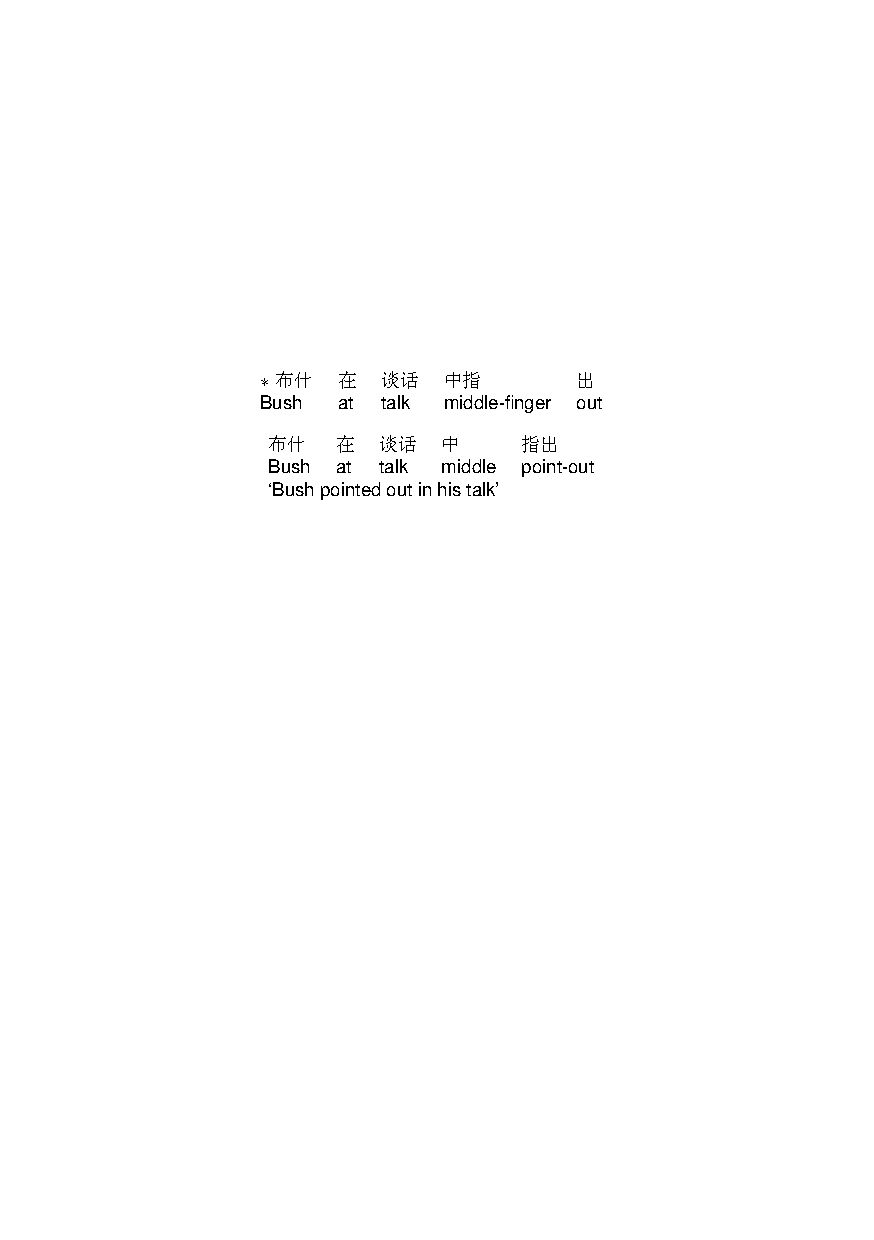
\includegraphics[width=.65\textwidth]{figures/chinese-bracketing-ambiguity}

\ea A potential overlapping ambiguity in Chinese.\\
  \label{exfig:chinese-tokenization}
\let\eachwordone=\cn
	\ea[*]{\gll 布什 在 谈话 中指 出\\
	Bush at talk middle-finger  out\\}

	\ex[]{\gll 布什 在 谈话 中 指出\\
	Bush at talk middle  point-out\\
	\glt `Bush pointed out in his  talk'}
	\z
\z

\let\eachwordone=\upshape
% \end{figure}



You may consider yourself lucky that the writing system used for
English makes it so much easier to determine what the words are by
simply starting a new word whenever there is a space. But even for
English, life is not that simple. After all, \exsent{inasmuch as} and
\exsent{insofar as} would then be split into two tokens and \exsent{in
  spite of} into three -- but to process them further or even just to
look them up in a dictionary, clearly identifying them as a single
token would be most useful! For an even more common case, let's start
with a simple sentence such as \REF{ex:car}, where starting a new
token for every word is straightforward.

\ea \ea \label{ex:car} I got my car fixed yesterday.
      \ex \label{ex:flu} I got my flu shot yesterday.
    \ex \label{ex:jacket} I got my jacket yesterday.
\z
\z 

If we hear \REF{ex:car}, we assume the speaker hired someone to fix their car.
But if we see \REF{ex:flu} on the lapel sticker of someone in the
street, we do not think that they hired someone to shoot their flu!
%not run away thinking we met a criminal bragging about his first killing! 
We immediately interpret \exsent{flu shot}
as a single token, parallel to occurrence of \exsent{jacket} in
\REF{ex:jacket}, even though it contains a space. Naturally,
this is very much language-dependent, as a \keyword{compound
  noun} such as \exsent{flu shot} is written
without spaces as \exsent{Grippeimpfung} in German. So spaces should
presumably be allowed in some English tokens, which immediately raises
the question of when exactly a tokenizer should identify words that
include spaces and when not.

The opposite problem is posed by strings such as \exsent{I'm},
\exsent{cannot}, or \exsent{gonna}. None of these tokens contains a
space, but we know that \exsent{I'm} is nothing but a short form, a
so-called \keyword{contraction}, of \exsent{I am}. Similarly,
\exsent{gonna} occurs in the same places and is interpreted in the
same way as \exsent{going to}. And a word such as \exsent{dunno}
(which might well appear in an English text to be processed even if
some prescriptive writing instructors would say not to use it) seems to be equivalent to
\exsent{do not know}. So, does it make sense to treat them as one token
in the contracted form and as two or three tokens in the form
including a space? Clearly, treating the two variants in such radically
different ways would complicate all later processing, which would not
be necessary if we, e.g., tokenized \exsent{I'm} as two tokens
\exsent{I} and \exsent{'m}. This naturally raises the general question of
when exactly a tokenizer should split up English strings that do not
contain spaces into multiple tokens.

In sum, processing text requires us to separate it into word tokens.  This task may seem straightforward in writing systems that use spaces; but even in English, there are challenging cases such as \textit{flu shot} (which contains a space but functions grammatically as a single noun) and \textit{dunno} (which contains no spaces but functions grammatically as three words, \textit{do not know}).  The challenges are even greater in writing systems that do not use spaces, such as Chinese, and in lower-resourced languages for which we can find less data to train an automatic tokenizer.  

Returning to CALL as an application, an intelligent CALL system needs to tokenize the L2 text in order to provide metalinguistic feedback on it.  Depending on the language and the writing system, that task might be more or less difficult.  Tokenization might also be harder in the free-text writings of L2 learners, who are still figuring out how to use the target language's conventions for spelling and spacing.



%In sum, to tokenize an English text, there are some general strategies, such as starting a new token whenever we encounter a space or punctuation symbol, and there are more specific segmentation cases where tokens can contain spaces and where multiple tokens result from a string lacking spaces. The automatic tokenizers used today thus typically contain long lists of known words and abbreviations, as well as a number of rules identifying common subregularities.


\subsection{Grammar and syntax}
% syntax 
% need to organize all this nonsense
% representing syntax could help with metalinguistic feedback.
% inflectional morphology.
% word order; word order OPTIONS; missing words, improperly present words.
% also to create more exercises... 
% or perhaps could prompt a language model to do so? depending on the status of generative AI in that language.

Once we have tokenized and part-of-speech-tagged the words of a language, it can also be helpful for an intelligent CALL system to create a syntactic representation for each sentence, using a dependency parser as introduced in \chapref{ch:writers-aids}.  Then, just as with the writers' aids discussed in \chapref{ch:writers-aids}, this representation could be used to provide metalinguistic feedback leveraging general insights about the grammar of the language. 

A syntactic representation could be used in a CALL system to offer helpful explanations of spelling errors (\chapref{ch:writers-aids}), for example correcting \exsent{*la casa rojo} in Spanish to \exsent{la casa roja} `the red house,' making sure that the adjective \exword{roja} `red' \keywordAs{agrees}{agreement} in gender and number with the noun \exword{casa} `house' that it modifies.  \exword{Rojo} is a real Spanish word, so the only way to identify it as an error is to recognize that its gendered suffix \exword{-o} mismatches with the gender of the noun \exword{casa} that it modifies. A dependency parse of this sentence could be used by the CALL system to flag the error and explain why \exword{roja} is the correct form.    

The gendered adjective endings in Spanish represent one type of \keyword{inflectional morphology} -- the way that a word changes form depending on its grammatical context.  Inflectional morphology also extends to verbs, which inflect in English for tense as well as agreement with their subjects, as in \exword{Holly swims}; a CALL system could use a dependency representation to explain why \exsent{*Holly swim} uses the prescriptively incorrect inflection.  Similarly, a dependency representation could be used to explain why \exsent{*Me love pizza} is incorrect: English pronouns take different forms (called \keywordAs{case}{grammatical case}) depending on their grammatical role in the sentence; \exword{I} is the \keyword{nominative} form used for grammatical subjects, while \exword{me} is the \keyword{accusative} form used for objects.  The structure and functions of such word forms are investigated in \keyword{morphology}, a subfield of linguistics. 

Beyond the form of individual words, a dependency representation could also be used in a CALL system to flag and explain errors in how the words are organized into a sentence.  As mentioned above,  if the learner writes  \exsent{*Maya shopped flowers for Juan}, an intelligent CALL system could explain that \exword{shop} does not combine with a direct object such as \exword{flowers}; if the learner writes \exsent{*Maya bought}, it could explain that \exword{buy} does need a direct object. 

Of course, to give such metalinguistic feedback, the CALL system would have to map a past-tense inflected form such as \exword{shopped} to the \keyword{lemma} (also known as the \keyword{citation form}) \exword{shop}, the form given in a dictionary or a list of intransitive English verbs. 


The grammar of a language is in some ways rigid (\exsent{Me love pizza} is rigidly ungrammatical in standard English), but also flexible in that it allows many options.  For example, the fill-in-the-blank exercise \REF{ex:fib-phrasal-verb} should allow the particle \exword{down} to appear right after the verb as well as at the end of the sentence.  An intelligent CALL system should allow such options not just for this exercise and this phrasal verb (\exword{turn down}), but for all exercises using any phrasal verb (\exword{set up, put in}, and so on).

\ea  \label{ex:fib-phrasal-verb} Maya, the radio is much too
  loud. Please \uline{\hspace{3cm}}!  
    \ea  turn down the radio. 
    \ex turn the radio down.
     \ex *down turn the radio.
    \z
    \z 



While phrasal verbs allow multiple grammatical options, the syntax of English is generally quite rigid: Sentences follow a strict Subject-Verb-Object word order (\exsent{Maya bought flowers}, not \exsent{*Bought flowers Maya}).  But other languages such as Russian and Latin allow \keyword{free word order}, using case-marking suffixes on nouns rather than word order to indicate their grammatical role.  In  \REF{latin}, we know that \exword{puella} `girl' is the grammatical subject of the sentence, no matter where it occurs, because it uses the nominative case marking.  \exword{Canem} `dog' is the object because it uses the accusative case.  A CALL system for Latin should allow all these options in the learner's writing.



\ea \label{latin}
    \ea \gll Canem puella amat \\
        dog-\textsc{acc} girl-\textsc{nom} love-\textsc{3sg} \\
        \glt{`The girl loves the dog.'}
    \ex \gll Puella amat canem \\
        girl-\textsc{nom}  love-\textsc{3sg} dog-\textsc{acc} \\
        \glt{`The girl loves the dog.'}
    \ex  \gll Puella canem amat \\
        girl-\textsc{nom}   dog-\textsc{acc} love-\textsc{3sg} \\
        \glt{`The girl loves the dog.'}
\z
\z 

The sentences in  \REF{latin} are \keywordAs{glossed}{gloss}, meaning that they are written in three lines such that the top line reflects the target Latin orthography; the second line offers a literal word-by-word translation space-aligned with the top line, including an analysis of case marking and inflection (\exword{nominative, accusative, third singular}); and the third line provides an ordinary English translation.  This format is used whenever linguists represent data from other languages.

All three options in \REF{latin} are grammatical, but one might be preferred over another depending on the larger context.  Generally \citep{ClarkClark:1977}, people prefer to follow the \keyword{given-before-new} principle, placing information earlier in the sentence when it is already related to the prior conversation, and later in the sentence when it introduces new individuals or ideas.  For a human or a computer to implement that constraint, one would need a rich representation of the discourse above and beyond the syntax of a particular sentence.

Returning to the value of syntactic representations for CALL, such tools could 
 also help the CALL designer to design further exercises efficiently.  For example, if the CALL system already uses the sentence \exsent{The girl eats the apple} in its question bank, it could automatically suggest further sentences by swapping out the noun phrase \exword{the girl} for any other noun phrase denoting an animate (living) entity --\exword{my dog, your brother}, and so on; or replacing \exword{the apple} with other vocabulary words from a unit on food (\exword{pizza, breakfast,} and so on).  Multiple-choice distractors could be automatically suggested from among other words in the same part-of-speech category as the target answer; perhaps the system could even use a language model (a fancier version of the $n$-gram probability model sketched in \chapref{ch:writers-aids}) to ensure that the distractors would result in a markedly less probable sentence than the correct answer, thus automatically recognizing \exword{pizza} as a better completion than \exword{phone} for \exsent{Your brother eats the\ldots}.  Leveraging such insights, an instructional designer could automatically generate a suite of questions and example sentences rather than writing each one by hand.

Expanding on the utility of language models, a generative language model could also be prompted to  offer metalinguistic feedback automatically, or to write further questions and example sentences.  For well-resourced languages such as English, such tools hold great promise for CALL because they are able to distill information about grammar from large-scale data even without making direct reference to explicit representations such as dependency parses.
For lower-resourced languages without generative language models, CALL designers may need to use more traditional handwritten exercises and feedback.  But in either case, distilling insights about the language helps an intelligent CALL system to give more general, flexible feedback across more diverse, unexpected input from the learner.



%Naturally, there are many abstractions and generalizations about language that can be used in concisely characterizing and providing feedback to learner answers in CALL systems. Another typical area in this context is \keyword{grammar} -- in a sense that is quite different from boring and dry rule books stipulating things. It is more related to the regularities you can observe in, say, chemistry, when you ask yourself what happens when you combine two given substances.  Certain molecules can combine; others don't; a particular order is needed for them to be able to combine; and sometimes an additional element, a catalyst, needs to be present for a combination to be possible.  Or if you think of music, there are clear generalizations about the way you can combine musical notes in chords or when setting music.  For those who like neither chemistry nor music, just think of the good old days when you may well have played with LEGOs -- and again only certain forms fit together in a particular order, independent of what it is that you actually want to build. So that is what grammar is about when it comes to using language.

% Grammar as studied in the linguistic subfield of \keyword{syntax} captures the same kind of generalizations for language. We already  mentioned some of the basic generalizations syntax makes in chapter~\ref{sec:what-is-grammar}. It includes generalizations about the \ind{word order}order in which words can occur. For example, in a typical English sentence, the subject precedes the verb and the object follows it. There also are generalizations about which elements have to appear together; for example, if the verb \exsent{devour} occurs in a sentence, it must be accompanied by a particular kind of an object, a noun phrase, to avoid ungrammatical sentences such as \exsent{*Maya  devoured recently} (in contrast to the acceptable \exsent{Maya ate recently}).  Here, the generalization is that a verb can \ind{selection}select (or \ind{subcatego\-riza\-tion}subcategorize) the category of elements which can or must accompany it: for reasons long debated by lexical semanticists, \exword{devour} requires a syntactic object, while \exword{eat} does not.

%Other generalizations in the area of syntax deal with the forms that words need to appear in to be able to occur together. For example, a subject can only appear together with a verb if they share so-called \keyword{agreement} features, a generalization which is necessary to rule out ungrammatical sentences such as \exsent{I walks.}  In other situations, when the generalization involves one element telling another what to look like, one typically speaks of \keyword{government}. For example, a verb such as \exsent{hug} requires its object to occur in accusative case, to ensure we get sentences such as \exsent{Sarah hugged him.} and not sentences where we instead get the nominative form of the pronoun, as in \exsent{Sarah hugged he.}

  
%For exercises where the learner can enter more than single words, we face an additional problem since, depending on the language, words are combined in different orders and forms to create sentences. This aspect of language is studied in the subfield of \keyword{syntax}, which identifies different word order possibilities and the forms in which words have to appear in these different patterns (see chapter~\ref{sec:what-is-grammar}). 



%These types of linguistic analysis can be leveraged to create a CALL system that is ``intelligent'' in the sense that it can provide metalinguistic feedback about such patterns.


%In ending this discussion, let us note that there are things we can say about the form in general, independent of the exercise. For example, we can refer to parts-of-speech and require that every sentence should contain a verb; then, we can connect that requirement to feedback reporting when a verb is missing. For such rules, the particular exercise they get applied to is no longer relevant, apart from the fact that the exercise requires a sentence as answer. If this idea of using rules sounds familiar, you are right: It is the approach of rule-based techniques to grammar checking we mentioned in section \ref{sec:grammar-checking}, used in the grammar and style checkers found in common word processing software today.



\subsection{Representations of meaning}

So far, we have explored how a CALL system can provide metalinguistic feedback about grammar. As another way that CALL tools can represent language, we introduce some simple tools aiming to capture not just structure, but meaning.

We saw above that a CALL system should allow multiple different word orders (\exword{turn down the radio, turn the radio down}) as correct answers, because English word order is flexible for phrasal verbs.  Similarly, a CALL system should allow many different answers to a question such as \REF{ex:november}, because all of these different formats \REF{nov1}--\REF{novend} refer to the same date.  (Americans prefer to write months before days, as in 11/6, whereas Europeans prefer the opposite order 6/11).

\ea \label{ex:november}Today is November 5. So tomorrow is \uline{\hspace{3cm}}. 
    \ea  \label{nov1} November 6.
    \ex the sixth.
    \ex  November the sixth.
    \ex  6/11.
    \ex 11.6.
    \ex \label{novend} 6 November.
\z 
\z 


Of course, if \REF{ex:november} were framed as a multiple-choice question, then the pre-determined answer choices could be hand-labeled as correct or incorrect; but if it is a free-text fill-in-the-blank question, then the CALL system would have to handle all the different possible formats for dates.  In language processing, dates are one example of \keyword{named entities}; they refer to specific real-world entities such as dates on a digital calendar. Other examples of named entities include names of people, companies, countries, addresses, and so-called \keyword{deictic} words such as \exword{today, tomorrow}, and so on, whose reference depends on the context in which they are used. The task of \keyword{named entity recognition} aims to identify such phrases in text, for example to help extract structured information (discussed further in \chapref{ch:searching}) from text, or to use digital assistants for scheduling purposes (\chapref{ch:dialog-systems}).  For CALL, named entity recognition would allow many different formats for a date to be understood as \keywordAs{synonyms}{synonym}.


At this point, one might object that the different ways of formatting dates is not a particularly interesting aspect of language learning.  But the goal of representing meaning is much more broadly useful.  For example, consider fill-in-the-blank exercise \REF{ex:fib-synonym}, modeled on a German exercise in the E-Tutor system of \citet{Heift:2010}.

\ea  \label{ex:fib-synonym} John works in New York City, but his
  family lives in Boston. On the weekend, he drives home. Fortunately,
  John has a new \uline{\hspace{2.5cm}}.
\z 

The possible correct answers go far beyond different formatting for dates.  For one thing, the possible correct answers include synonyms such as
\exsent{car} and \exsent{automobile}. And as we discuss in the context
of machine translation in Chapter~\ref{ch:mt}, there are various other \keywordAs{lexical semantic relations}{lexical
  semantic relation} between words.  In our context, another relevant
lexical semantic relation is hyponymy; this is the option of picking a
more specific term, a so-called \keyword{hyponym}, such as \exsent{pick-up}, \exsent{SUV}, or \exsent{Volkswagen} in place of the
more general term \exsent{car}, the \keyword{hypernym}.  Finally, though the people designing exercises generally try to avoid this,
there may also be multiple different meanings that make sense for a
slot in a given exercise; in \REF{ex:fib-synonym} the context
would also be compatible with inserting \exsent{helicopter} or even \exsent{audiobook} (to listen to in the car!) -- and for each one of them, various semantically related words could be used.

Rather than simply trying to brainstorm all possible answers for  \REF{ex:fib-synonym}, an intelligent CALL system could count any vehicle-related words as correct, either by using a hand-built resource such as WordNet \citep{fellbaum:98}, which represents hypernym and hyponym relations, for example specicifying that trucks and cars are vehicles; or a representation learned bottom-up from text in ways to be explored further in \chapref{ch:textasdata}. 

%Clearly specifying all such related words as options in the frame of a FIB exercise would involve a lot of work -- and this is work that would have to be repeated for every new exercise, even though these lexical semantic relations are encoding a general property of the language, not something specific to a given exercise.



%Many languages include an even richer inventory of forms than English. For example, some of you may know from the study of Spanish that verbs surface in complex conjugation patterns. For example, just looking at the present tense of one of the verbs meaning \exsent{to   be} in Spanish, one finds the six forms \exsent{soy}, \exsent{eres}, \exsent{es}, \exsent{somos}, \exsent{sois}, \exsent{son} -- and this is only one of over a dozen other tenses and moods.  If we want to specify an exercise frame in a CALL system to provide different feedback for different forms, we would have to spell out the many different forms for each exercise -- even though this clearly is a general property of the language, which we should be able to encode once and for all, instead of having to spell it out for each exercise frame.

% So far, we have considered the question of how we can make use of linguistic generalizations to compactly specify the expected correct or incorrect answers, instead of spelling out all forms and word orders by hand in the frame of a given exercise. We still have to specify in the frame what we expect to find in the response, but we can do this more compactly if we can rely on natural language processing (NLP) tools to generate or recognize the wide range of morphological forms and word orders for us.  In other words, we can compactly specify the different form options by which language can encode a given meaning, but we still need to provide some specification of the intended answer to ensure that the learner actually provided a meaningful answer to a given exercise.



\subsection{Types of CALL exercises}

Having explored some text-processing tools used in CALL, we turn to the types of questions typically used in CALL systems.  For each one, it is useful to consider: How would a CALL system automatically recognize the learner's answer as correct?  What sorts of metalinguistic feedback could be given for incorrect answers?  How could text-processing tools or generative language models be used to create further questions?  Finally, how difficult is each type of question -- for a CALL designer to write, for a CALL system to grade; or for a learner to complete correctly?  Turning from the language to the learner, which questions will be most useful, fun, or frustrating for them?


 \begin{itemize}
     \item Matching a (spoken or written) word in the L2 to an image or a translation in the learner's L1, or vice versa.
     \item Fill-in-the-blank exercises where a learner has to complete a sentence with an appropriate missing word or provide the correct form/conjugation of a given lemma.  These could take the form of multiple-choice or free-text-box exercises.
         \item Given a set of options, choosing the one that constitutes the most sensible reply to a previous conversational turn.
     \item Testing the comprehension of spoken or written material through true-false or multiple-choice questions.
     \item Dictation exercises, where the learner is asked to transcribe a sound clip -- using a word bank or a free-text box.
     \item Pronunciation exercises, where the learner is asked to say something into a microphone, graded for accuracy via a speech-to-text system.
     \item Translation exercises, where the learner is asked to translate from the L2 to the L1 or vice versa -- with a word bank or a free-text box.
     %Such exercises are easier when going from the L2 to the L1, and when the learner is provided with a bank of words to arrange; it is much harder for the learner to translate the L1 to the L2 in a free text box, and perhaps also harder for a CALL system to grade it.
     \item Correct-the-error exercises, where a learner is asked to select an erroneous word in a sentence that they are given.
     \item Open-ended free-text or free-speech questions, like \exsent{Hello, welcome to our caf\'e, what would you like to order?} or \exsent{What was your favorite part of this story?} -- to be graded for length, grammatical correctness, and whether the learner's answer makes sense in context.
 \end{itemize}



%(these are generally finite-state rules; see Under the Hood~\ref{uth:fsas} for a discussion of finite-state technology). - this under the hood was removed sorry! - LG



%We already discussed the techniques used for expressing generalizations about the order and form of words in section~\ref{sec:grammar-checking} in the context of the chapter on Writers' Aids, so we will not repeat them here and instead continue by asking ourselves what happens when we add linguistic analysis in the form of tokenization, part-of-speech tagging, and syntactic parsing and agreement checking to a CALL system. We then obtain a CALL system

%-- for example, there is no way to guess the names of the people a question asked about based on properties of the language alone.



% part of speech -- need to know parts of speech to create distractors, metalinguistic feedback, perhaps to automatically write sentences using vocabulary items, know which words can be substituted for which others 
% which requires tokenization 
% named entity recognition - perhaps useful for grading free text exercises?
% hypernyms and stuff  - also perhaps useful for grading free-text exercises 
% morphology, lemmas 

% represent grammar, give specific metalinguistic feedback like writers aids, tell people e.g., adjectives have to agree in gender with nouns; this verb needs an object; etc.
% perhaps not easy when the sentence itself may have somewhat nonstandard grammar, to be choiced for a job





\section{Modeling the learner}

CALL systems aim to model not just language, but also learners and learning.  Here, we explore how CALL tools can represent exercises and learners to offer the most motivating and helpful curriculum for each learner.


\subsection{Sequencing of material}

At the most rudimentary level, a \keyword{linear CALL system} would give all students the same exercises in the same order.  Even here, we face design choices: If a student gets a question wrong, should they still just move to the next question, or should they get another chance to get it right before proceeding?  Either way, a linear CALL system runs the risk that advanced students may get bored, and struggling students may feel overwhelmed.  

In contrast, in \keywordAs{branching CALL systems}{branching CALL system}, the sequencing of the exercises depends on what the
student does. If a student answers one question right, the system offers a slightly
harder question; if the student gets it wrong, the
system reverts to a simpler question and might provide additional
feedback or practice related to the student's mistake. Like giving each student their own one-on-one tutor, a CALL system could offer instruction precisely tailored to learners' individual needs. 

This type of \keyword{dynamic sequencing} is also used in \keywordAs{computer
adaptive testing}{computer adaptive testing (CAT)}, such as the GRE (Graduate Record Examination, offered by the Educational Testing Service).  Here too, the sequence of questions depends on the test-taker's previous answers. But this time, the goal is different: If the system can make
sure that strong students do not spend time on questions that are much
too easy for them, and weak students do not spend time on questions
that are much too hard, then it will be able to assess each student's ability accurately using fewer questions and less time.  This adaptive strategy is only feasible if the test is delivered electronically.

To sequence questions dynamically by difficulty, a CALL system would have to associate each question with a difficulty level -- perhaps the level that it targets according to a metric of L2 success such as the ACTFL or CEFR scales mentioned above; a unit in the course curriculum (Level 3 Spanish); or -- leveraging the CALL system's own usage data rather than a human-assigned label -- the percentage of learners (overall or at a given level) who get it right.

% -----------------------------------------------------------------------------


%In their most basic variants, \keywordAs{linear CALL systems}{linear  CALL system} pose a question as part of an exercise, accept an answer from the student, and then inform the student as to whether or not the answer was correct (as well as any more detailed feedback stored for the choice made). Regardless of the correctness of the answer, linear systems then proceed to the next question in a pre-determined (\exword{linear}) lineup.



\subsection{Characteristics of individual learners}

In addition to modeling the target language and the difficulty of each exercise, it is also useful for a CALL system to represent information about the individual learner.  This endeavor is known as \keyword{learner modeling}.

For one thing, a given learner is associated with more or less stable properties such as their L1 and their motivation for learning the L2 (school, travel, immigration, and so on).  Other relatively stable properties might include their technical setup (whether they use a desktop or a mobile phone; whether they avoid talking out loud because they are doing their CALL exercises in a silent library); their preferred learning style (whether they want to focus on speaking or writing, whether they enjoy longer stories or quick flashcards).  Some of these learner traits might be inferred from how the learner interacts with the CALL system, but others could be gathered through a survey when they sign up.

Then a CALL system could customize itself to these traits, for example focusing on travel vocabulary for future travelers, or avoiding speech-to-text exercises for people who don't have a sound setup.  More importantly, the L1 of the learner strongly influences the mistakes that they might make when learning an L2.  For example, languages such as Chinese and Czech do not use determiners (also called articles; \exword{the, a}), so English learners from those L1 backgrounds may need more feedback and exercises related to determiners.  For an English learner from a determiner-using L1 such as German, though, the absence of a determiner might be a minor typo, so perhaps it should not be emphasized as much by the CALL system. In other words, tutoring systems are often designed to focus on the learner's most important errors rather than overwhelming them with dozens of corrections at once (\keyword{prioritization of feedback}).

Of course,  L1 transfer can also be helpful, as when learners can take advantage of cognates shared across languages (English \exword{coffee}, French \exword{caf\'e}).   Thus, modeling each learner's L1 can be used to tailor the CALL curriculum to their strengths as well as their areas for improvement.

%For the second component of learner modeling, on the other hand, the system needs to draw \keywordAs{inferences}{inference} from the learner's interaction with the system.  Let us take a closer look at what is meant by inferences here and why they are needed.


Beyond the learner's stable personal traits, a CALL system might also analyze their dynamic interactions with the CALL system -- the questions they get right and wrong; the number of days and minutes per day they have spent learning; and the words and structures they seem to know versus the ones they struggle with.  To draw inferences about a learner's knowledge of structure, a CALL system has to abstract away from specific questions/answers to distill information about both the learner and the structure of the language. 

For example, one might want to assess whether a learner knows present-tense subject-verb agreement (in English, \exsent{I swim} versus \exword{Maya swims}).  If so,  the CALL sequence could move on to more advanced topics; if not, it could offer further instruction.  If they have clearly mastered subject-verb agreement but seem to get it wrong unexpectedly, perhaps the CALL system should take this error as a typo rather than a true confusion (echoing the discussion of spelling errors in \chapref{ch:writers-aids}).  

But it is not trivial to infer from a learner's behavior whether they have learned a target pattern such as subject-verb agreement.  To draw such an inference, each question would have to be labeled (perhaps automatically) for the patterns that it tests.  For intelligent tutoring as well as \keyword{language testing}, instructional designers have to be wary of \keyword{construct under-representation} -- drawing incorrect inferences when the learner has not answered enough questions to assess what they truly know, for example inferring that they know subject-verb agreement when they just made a lucky guess in a multiple-choice question.  This problem can only be avoided by giving the learner more questions pinpointing the target knowledge.



% It is far from trivial to determine when such inferences are valid. Just like in the context of \keyword{language testing}, in the intelligent tutoring context, \keyword{construct under-representation} can hinder the recording of a particular ability in a learner model. In other words, the exercises which the student is completing need to provide enough evidence for a particular language ability if we want to record and update the record of what the learner can do in the learner model. 

% Construct underrepresentation (CU) occurs when the examination lacks validity because the examination content is not reflective of relevant knowledge

To ensure valid inferences, it also is not enough
to consider the learner's answers themselves. Instead, we also need
to include information on the exercise the learner was completing and
the strategies learners may employ to succeed in such a task. For
example, a particular learner answer may simply have been copied from the context of the question, which is
known as \keyword{lifting}. A student who responds with \REF{liftex} might not be truly confident in creating relative clauses (\exsent{places I've visited}) if they are just lifting that phrase from the question.

\ea \ea   What is your favorite place you've visited?
    \ex  \label{liftex}  I like many places I've visited.
\z 
\z 

To be able to interpret learner answers in terms of what they allow us to infer about the learner's abilities, an intelligent tutoring system thus also needs to take into account \keyword{learner strategies} such as lifting or avoiding structures that the
learner is unsure about.

Such inferences constitute one example of learner modeling.  More broadly, by amassing data on what the learner gets right and wrong, a tutoring system can draw inferences about the words or grammatical structures they can understand; the words or grammatical structures they can produce spontaneously; the probability of them answering a given question correctly; the maximum length or difficulty level of a sentence that they can write/translate correctly; the probability of them quitting or persevering; the amount of time they will choose to spend learning; and so on.   The tutoring system could customize the curriculum to these traits, for example offering exercises to each learner that they have about an 80 percent chance of getting right.  Of course, harder exercises can be both instructive and discouraging, and easy exercises can be both boring and affirming, so CALL researchers analyze learner data to strike the right balance.

In sum, in modeling both language and learners, intelligent CALL systems also have to model both general and specific facts.  CALL systems model general facts about the structure of the language as well as how those facts are manifested in specific exercises to be sequenced, tagged with the words/structures that they test, and associated with metalinguistic feedback.  They also represent general facts about how L2 learning progresses along with specific inferences about the progress, preferences, strengths, and weaknesses of individual learners drawn from the history of their interaction with the CALL system.  The key to success lies in synthesizing all this information to create the most effective and enjoyable system.



%Concluding our exploration of Language Tutoring Systems and the role the analysis of language needs to play in it, the use of NLP in language teaching and in education in general is one of the application areas that is just starting to take off. Following on the footsteps of the first few intelligent language tutoring systems in real-life use today (E-Tutor, Robo-Sensei, TAGARELA, FeedBook), 

%the next years will bring a much wider range of exercise types with more adaptive feedback and increased use of virtual environments.  The first interactive robots used for language teaching are already appearing on the scene. Based on what we discussed in this chapter, it is clear, though, that one aspect will stay the same in all such uses of computers in language learning: for such systems to be able to react to learner input in an intelligent way, going beyond a small number of preenvisaged frame specifications, it is crucial for the systems to be able to step back from the specific learner answer at hand to more abstract linguistic representations. Such representations support system feedback and interaction to a wide range of learner responses. 


%For example, one may want to record whether a learner answer contains a finite verb and whether it showed correct subject-verb agreement. Once we have observed learner answers including instances of a particular linguistic class or relation, we can infer that the learner has mastered this aspect of the language to be learned and, e.g., deprioritize feedback on it in the future.  Where the tutoring system supports this, learner models may also be used to \keywordAs{sequence   the teaching material}{sequencing of teaching material} appropriately, e.g., by guiding learners to additional material on concepts they apparently have not mastered yet.

% One naturally could simply record everything the learner enters in exactly the way it is entered. But all this would help us detect is whether the learner has entered a particular answer before, which would allow the system to provide specific feedback for a single, very specific case of minor relevance.  To be able to make more use of recording the past learner performance, just like in the discussion of analysis and feedback in the first part of the chapter, it is necessary to abstract away from the surface of what the learner entered into the system to the more general linguistic properties and classes for which the learner answer provides evidence.




%So far, we have mentioned two sources of information which are used by computer-assisted language learning systems. We started with the information explicitly specified in the exercises, in particular the frames which need to be specified for each exercise in a traditional CALL system. The second source of information arises from the computational linguistic analysis in an ICALL system, which is based on the general knowledge about a language and thus is independent of a particular exercise. 



%In addition to those two sources of information -- the exercise and the language -- it can also be important to take into account what we know about the learner.  Generally speaking, such \keyword{learner   modeling} includes two types of information.  On the one hand, there are learner properties which are more or less permanent, such as the gender, native language, or learning style preferences -- and it is easy to see that, for example, system feedback for visual learners should be enhanced with more visual cues than for other learner types.

% On the other hand, there is the dynamic record of the learner performance so far, essentially a history recording whether a given learner successfully used particular words or structures before. Both types of information about the learner are relevant when providing feedback. 


%An important difference between the static learner properties such as their L1 and the constantly updated history of the learner interaction as the second component of learner modeling lies in the way in which the learner information is obtained. Information for the more or less permanent part of a learner model typically stems from a questionnaire asking for information such as their mother tongue, time spent abroad, other languages spoken in the family, as well as from tests providing information on the learner's general academic abilities or specific language abilities. 



% These exercises can be \keyword{dynamically sequenced} (presented in an order automatically adapted to what the learner does) so that the learner can be asked to repeat questions that they previously got wrong, or move on to more advanced exercises when they master simpler ones.    In a \keyword{branching} system, a learner might skip ahead to harder exercises if they get all the simple ones right, similar to the \keyword{computer-adaptive testing} used by some standardized tests.  These techniques would require every exercise to be associated with a difficulty level as well as perhaps an annotation of the skills and vocabulary that it tests, so that the tutoring system can tailor the exercises to each learner.




\section{Example: FeedBook}

To illustrate how CALL systems actually work, we explore the example of FeedBook, an \keyword{intelligent language tutoring system (ILTS)} developed at the University of T\"ubingen \citep{Rudzewitz-etal:2017,Meurers-etal:2019}, based on an official textbook for seventh-grade English in Germany.  It is called FeedBook because it augments the textbook with intelligent, individualized metalinguistic feedback.  

The exercises are inspired by \keyword{task-based language learning} -- the idea that students should learn to use the L2 to accomplish authentic tasks in context, such as booking travel or stating one's opinion about a news article, rather than simply drilling words and rules in the abstract.  But the exercises also target specific grammatical forms of the L2.  Therefore, FeedBook is built to provide feedback on both form and meaning.
% developed from a paper workbook for 7th grade English
% supposed to complement a teacher, help automate homework feedback (which is a more generally useful idea), also sort of works as a learning management system like Canvas or Blackboard, sends reminders about overdue work and so on.
% task-based language learning, task-based instruction

% Exercises are embedded in a meaningful context. Compared to traditional decontxtualized ``drill-and-kill'' exercises, such activities are more motivating for students and the abilities are more readily transferable to authentic, functional use of language as the overall learning goal. The pedagogical goal of these exercises, however, is the mastery of the use of certain forms of the language. Correspondingly, the system provides feedback on the correct realization of the appropriate form. An example for such \keyword{focus-on-form feedback} is shown in Figure~\ref{fig:feedbook-focus-on-form}.

Looking first at feedback on form, in \figref{fig:feedbook-focus-on-form}, the learner sees information about two options for a flight to Greece.  Which flight would they choose, and why?  In a free-text box (parallel to a written response on a paper homework assignment), the learner has written \REF{expensiver}.  Here, a pop-up box responds with \REF{corrxn}. 

\ea \ea \label{expensiver} *The tickets at Air-Con are expensiver than at Midair.  
\ex \label{corrxn} When an adjective has three or more syllables, we form the \keyword{comparative} with ``more'' and the \keyword{superlative} with ``most.''
\z
\z



The student has an opportunity to rate this feedback as \exword{hilfreich} `helpful' or not; then they have a chance to revise their answer.  Here, the feedback does not just say that something is wrong, nor does it provide the full solution (which might be optimal for a grammar checker for native speakers, as discussed in \chapref{ch:writers-aids}).  Instead, FeedBook gives a hint by explaining the general pattern that the learner is missing, which the learner can then apply to the specific word \exword{expensive}, so that the learner  has to consider the pattern and apply it themselves.


\begin{figure}
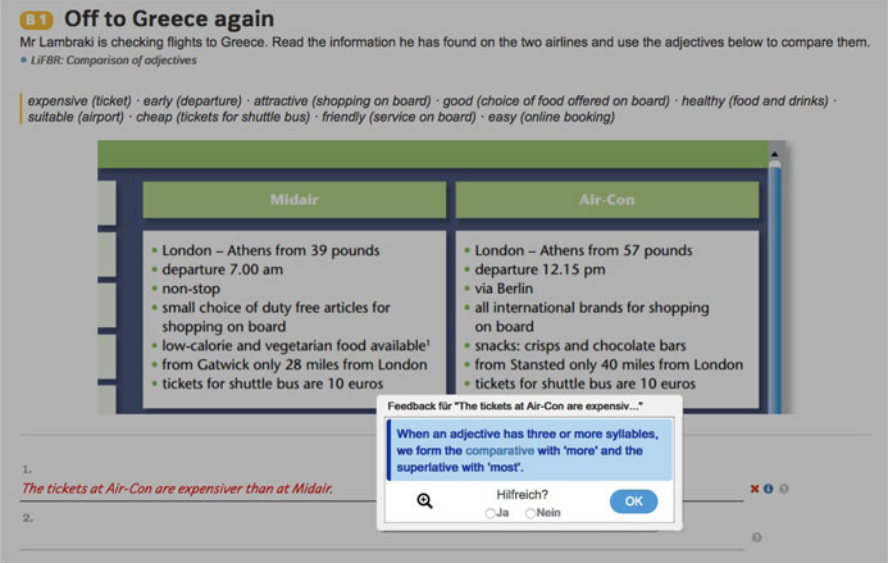
\includegraphics[trim=0 0 0 90,clip,width=0.7\textwidth]{figures/expensive_feedbook.png}
\caption{FeedBook: ``Focus on form'' feedback.}
\label{fig:feedbook-focus-on-form}
\end{figure}


As for feedback on meaning, in \figref{fig:feedbook-focus-on-meaning}, the learner sees a multi-paragraph autobiographical narrative about a kayaker, and is asked an open-ended comprehension question \REF{james}.  The learner has written \REF{student};  FeedBook has replied with \REF{missing}. 

\ea \label{james} How did James feel when he first came to St David's?
    \ea \label{student} James was a student.
    \ex \label{missing} There seems to be important information missing in your answer. Please have a look at the highlighted passage in the text.
\z
\z

The beginning of the narrative is highlighted in green, including the sentence \exsent{I wasn't very confident when I first arrived}.  Again, FeedBook does not just say that the answer is wrong, nor does it give the correct answer; instead, it gives a hint by narrowing down the long text to the portion containing the answer.  The student still has to figure out for themselves that \exsent{when I first arrived} aligns with \exsent{when he first came to St David's}, and that \exsent{I wasn't very confident} answers the question \exsent{How did James feel?}  The exercise becomes more manageable, but the learner still has to use their brain.

\begin{figure}
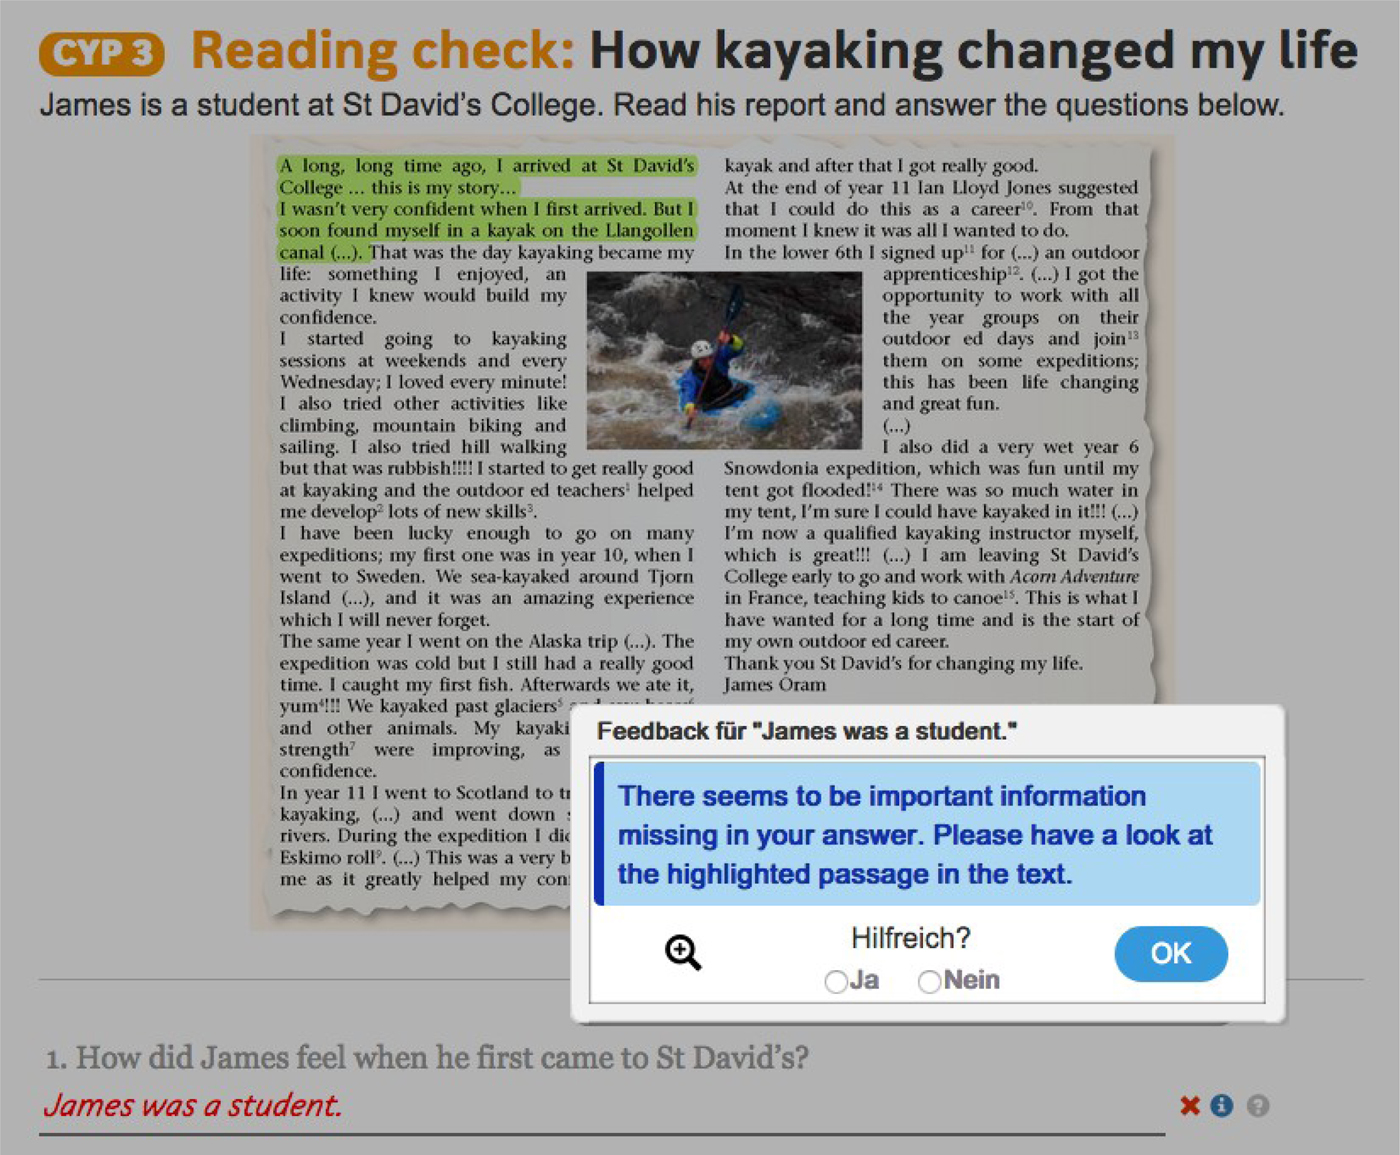
\includegraphics[trim=0 0 0 50,clip,width=\textwidth]{figures/kayak_feedbook.jpeg}
\caption{FeedBook: ``Focus on meaning'' feedback.}
\label{fig:feedbook-focus-on-meaning}
\end{figure}


FeedBook aims to supplement rather than replace an in-person class with a live teacher.  Whereas teachers historically had to correct students' work by hand and then return it to them days later, FeedBook provides immediate grading and feedback at scale, so that the teacher can focus on preparing the in-person class sessions.  FeedBook also functions as a \keyword{learning management system} such as Canvas or Blackboard (used in schools as a platform for course material, homework, grading, discussions, and so on), in that it sends reminders about missing homework to students and compiles statistics for the teacher on what students know and don't know.  Whereas the earliest such \keyword{intelligent tutoring systems} were built for math instruction, where students' answers are more constrained (i.e., to numerals), FeedBook leverages language technology to handle the unconstrained domain of language.  


% it's sort of like a smart textbook and also a learning management system.....
% these used to be harder for language than for stuff like math but NLP tools make it better.... right so say that.

%\begin{figure}[htb!]
%\includegraphics[trim=0 0 0 50,clip,width=\textwidth]{figures/2B1-incidental}
%\caption{FeedBook: ``Incidental focus on form'' feedback.}
%\label{fig:feedbook-incidental-focus-on-form}
%\end{figure}

% called TAGARELA
% (Teaching Aid for Grammatical Awareness, Recognition and Enhancement
% of Linguistic Abilities), an intelligent web-based workbook for
% beginning learners of Portuguese.

% The TAGARELA system offers self-guided activities accompanying
% teaching.  It includes six types of activities: listening
% comprehension, reading comprehension, picture description,
% fill-in-the-blank, rephrasing, and vocabulary. It thus is similar to
% traditional workbook exercises, with the addition of audio. But it
% provides on-the-spot meta-linguistic feedback on orthographic errors
% (spelling, spacing, punctuation), syntactic errors (nominal and verbal
% agreement), and semantic errors (missing or extra concepts, word
% choice).

% Figure~\ref{fig:missing-verb-feedback} shows a rephrasing activity, in
% which the learner is given a sentence and has to rewrite it using the
% words provided.
% \begin{figure}[htb!]
% 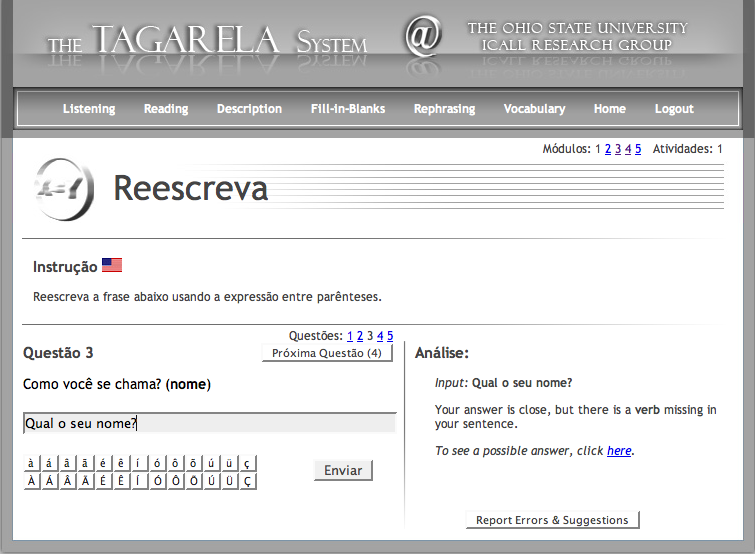
\includegraphics[trim=0 0 0 0,clip,width=\textwidth]{figures/MissingVerb}
% \caption{TAGARELA: Feedback on missing verb}
% \label{fig:missing-verb-feedback}
% \end{figure}\enlargethispage\baselineskip
% In this example, the learner forgot to include a verb in the answer
% they typed in the answer field at the bottom left of the page. The
% system displays a feedback message pointing out this error at the
% bottom right of the page. Note that just as discussed at the end of
% section~\ref{sec:call-aware}, a sentence missing a verb is an error
% the system can detect and provide feedback on solely based on
% knowledge about the language. In TAGARELA, this knowledge about the
% language is encoded in grammar rules for Portuguese, which are
% independent of this particular activity.

% Figure~\ref{fig:agreement-feedback} shows an example for a reading
% comprehension question.
% \begin{figure}[htb!]
% \includegraphics[trim=0 0 0 0,clip,width=\textwidth]{figures/Agreement}
% \caption{TAGARELA: Feedback on agreement}
% \label{fig:agreement-feedback}
% \end{figure}
% The feedback provided by TAGARELA for the learner response in this
% exercise illustrates another general type of error made by language
% learners, so-called \keywordAs{subject-verb agreement
%   errors}{subject-verb agreement error} where the form of the verb
% does not agree with its subject.

% The feedback in the previous two examples was computed by TAGARELA
% based on the system's general NLP capability to analyze language --
% from identifying tokens, words, lemmas, and part-of-speech to
% syntactic generalizations -- without the need for explicit frames
% spelling out all potential learner answers and the feedback to be
% provided. Yet we also mentioned at the end of the previous section
% that some of the feedback an ICALL system provides remains based on
% the specific exercise. An example for such exercise-specific feedback
% is shown in Figure~\ref{fig:exercise-specific-feedback},
% \begin{figure}[p]
% 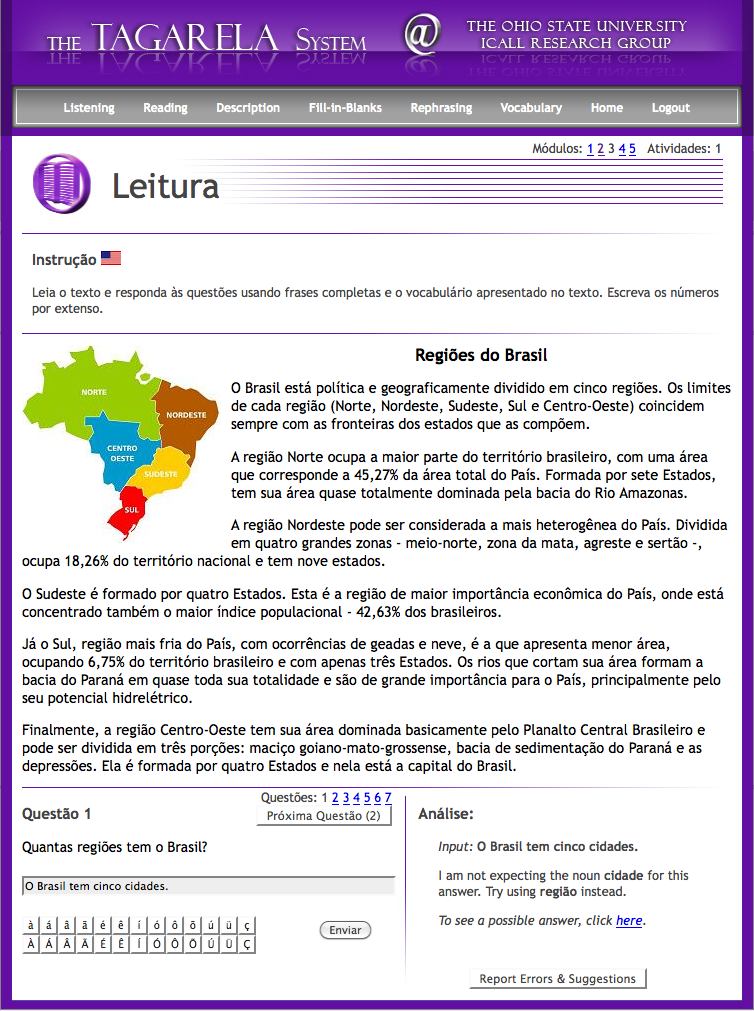
\includegraphics[trim=0 0 0 0,clip,width=\textwidth]{figures/reading-wrong-noun}
% \caption{TAGARELA: Example for exercise-specific feedback}
% \label{fig:exercise-specific-feedback}
% \end{figure}
% where a text about Brazil introduces the different regions of the
% country and the learner is asked a reading comprehension question
% about it.

% The learner response states that there are five cities in Brazil, even
% though the specific question at hand in this exercise was asking about
% the number of regions in that country. The system feedback alerts the
% learner of the fact that the answer is not expected to be about cities
% but about regions, which makes use of information specific to this
% exercise.

% Note that even for such feedback based on exercise-specific
% information, the feedback at the same time also makes use of
% generalizations detected by the system's NLP capabilities, by pointing
% out that the problem is associated with a noun. The system thus
% recognized the unexpected word \exsent{cidade} as belonging to the POS
% category noun and used that general information obtained about the
% learner input in formulating the feedback.

% -----------------------------------------------------------------------------

% \newpage






\section{Example: Duolingo}

As an example of a very popular language tutoring system, we turn to Duolingo, which offers online language lessons.

\subsection{Duolingo as a business}

Duolingo was founded in 2009 and released to the public in 2012 by Luis von Ahn, a Guatemalan-American computer science professor, and Severin Hacker, a Swiss graduate student, both at Carnegie Mellon University.  Luis von Ahn had previously founded ReCAPTCHA, a web verification tool for distinguishing humans from bots by asking them to transcribe a few characters of text from an image, which -- in an attempt to kill two birds with one stone -- was used to digitize portions of old books and newspapers that were too illegible to be processed automatically.  Duolingo was originally designed around the same two-birds-one-stone idea, aiming to teach people L2s while also gathering translations for the web, but the translation portion was eventually abandoned to focus on L2 teaching alone.

As of 2023, Duolingo claims to have been downloaded over 500 million times, with 4.2 million paid premium users and 54 million monthly active users.   Duolingo offers 43 different languages in over 100 different L1/L2 pairings.  Courses for lower-resourced languages are shorter and not as fully developed, but Duolingo advertises as a point of pride that they teach minority languages such as Navajo, Hawaiian, and Irish.  They even offer \keyword{constructed languages}, those consciously crafted as part of a fictional world-building exercise: Klingon (created for the television show \exword{Star Trek}), High Valyrian (from \exword{Game of Thrones}), and Esperanto (invented with the goal of fostering global understanding and peace).  Globally, the most popular language on Duolingo is English, followed by Spanish and French; in the United States, it is Spanish followed by French or, in some states with high immigration rates, English.  

Duolingo uses a \keyword{freemium} business model.  The free basic version cuts the learner off after they make five mistakes in a session and makes them watch ads, while the paid premium version allows unlimited mistakes, no ads, and offline lessons.  Duolingo can be considered a form of \keyword{edutainment} because it tries to \keyword{gamify} language learning.  Learners can follow friends, congratulate one another on their progress,  jockey for positions on a leaderboard, maintain their ``streak'' (number of consecutive learning days), earn points to spend in an online store (to buy an additional lesson on flirting, or to miss a day without losing their streak), and win badges to be shared on social media.  Duolingo is also notorious for sending persistent push notifications and emails (sent at the time of day when each learner usually logs on!) to keep learners coming back every day.  In other words, Duolingo is optimized not just for language learning, but equally for \keyword{user retention}.


\subsection{How does Duolingo teach language?}

Duolingo is organized into five-minute lessons of about 17 questions each.   Each lesson automatically self-extends to give the learner another chance at what they got wrong, and the lesson is only complete when all questions have been answered correctly.  Lessons are organized into topics (content topics such as greetings, travel, clothing, and current events; and grammar topics such as pronouns, future, past, and so on) and difficulty levels.  In the L1-English-to-L2-Spanish course, for example, the first level of a lesson on clothing might focus on matching words to pictures of clothing, and translating sentences from Spanish to English with a word bank, while further levels of that lesson would emphasize translating the same sentences from English to Spanish, first with a word bank and later into a free text box.  In addition to matching and translation, the questions also involve multiple choice, comprehension questions for text and audio, fill-in-the-blank, dictation, and repeating sentences out loud.  Even for exercises involving text rather than speech, the app plays text in the L2 out loud (leveraging text-to-speech tools) so the learner sees and hears it at the same time.  To move to the next level of a lesson, the last portion of each level requires the student to review their previous mistakes until they can answer them all correctly.  If a learner makes no mistakes on an early level of a lesson, the premium version of Duolingo allows them to skip to the next level.  


The lessons are organized into units, each one ending with a test that the learner must pass to unlock the next unit.   For learners who already have some experience with the L2, Duolingo offers a placement test so that they can skip the units that they already know. Early units focus on greetings, basic vocabulary, and simple grammar such as the present tense, while more advanced units use sentences about politics, religion, and complex grammar such as the subjunctive and \exword{not only \ldots but also}.  Some lessons start with an optional section of grammar tips, where a grammatical rule is stated explicitly and illustrated with examples. Leveraging language-aware generalizations, the same grammar tips recur as feedback if a learner makes a mistake on that grammatical pattern.  

%When a learner logs on to Duolingo, they have many different options for how to maintain their learning ``streak'' that day. They can choose any lesson in the units and levels that they have unlocked, for example choosing to advance in the  lesson on travel or start a new lesson on food.  They can take a test to try to advance to a new unit, review lessons that they already completed, practice previous mistakes, or focus on ``stories'' (short dialogs between Duolingo's diverse cast of animated characters, interspersed with exercises in comprehension and dictation).   Within a lesson, they sometimes have the option to earn additional points by doing the lesson in Hard Mode, with more free text boxes and L1-to-L2 translation exercises.    All  these options are intended to keep learners motivated by giving them autonomy.  

Within a lesson, the variety of question types (matching, fill-in-the-blank, multiple choice, dictation, saying a sentence out loud, different types of translation exercises) are chosen to keep learners engaged, and sequenced so that the hardest exercises come at the end of the lesson when a learner is least likely to give up.  If a learner makes multiple mistakes in a row, Duolingo fosters a growth mindset with encouraging messages about how making mistakes is part of learning.  The lessons feature cute animations of Duolingo's characters, each associated with their own voice, and correct answers are rewarded with a pleasant chiming sound plus an animation of one of the characters dancing or celebrating.  In all these ways, Duolingo is designed around the idea that a learner's attitude matters.

In contrast to the long text-comprehension questions used by FeedBook, Duolingo's exercises are much shorter and simpler, constrained by the size of a phone screen.  Because FeedBook is assigned by schools while Duolingo requires self-motivation, perhaps Duolingo's users are more likely to give up and thus prefer their work to be bite-sized.



\begin{figure}[htb!]
  \centering
  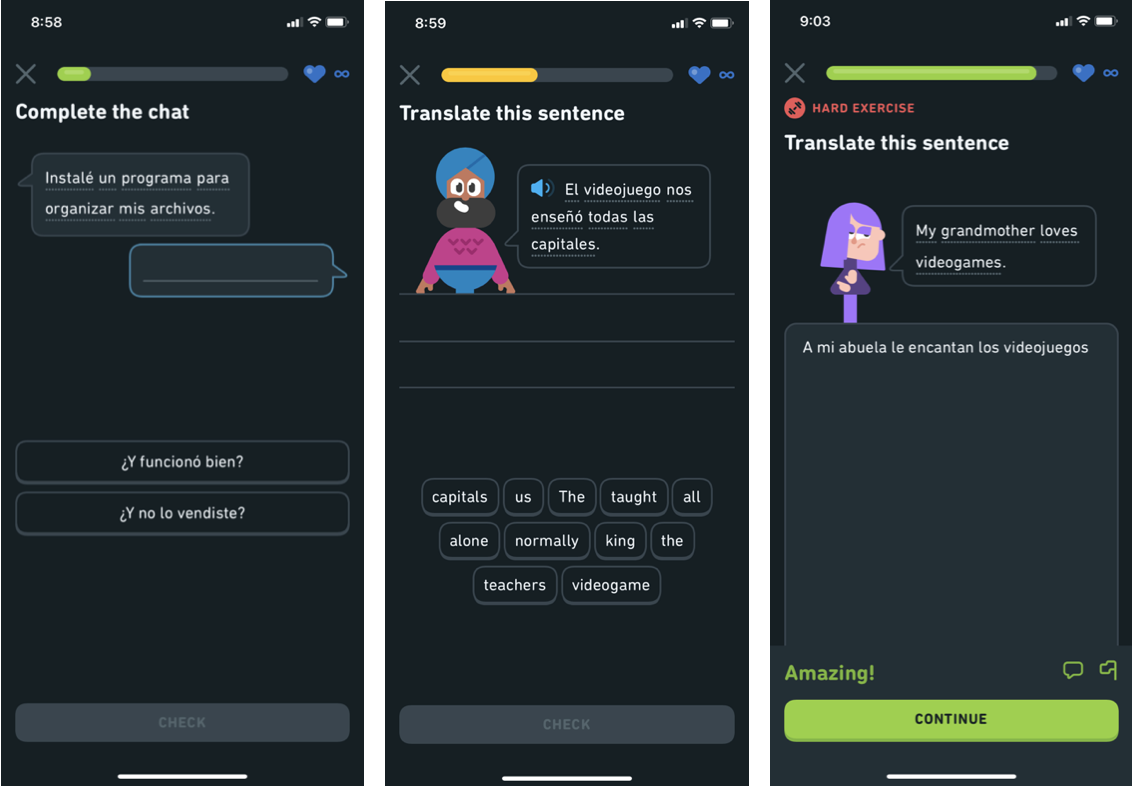
\includegraphics[width=\linewidth]{figures/duolingo_screenshots.png}
\caption{Screenshots from the Duolingo Spanish course: A multiple-choice comprehension question; a translation question from the L2 to the L1, with a word bank; and a translation question from the L2 to the L1, with a free text box.  As indicated by the progress bar, the questions get harder as the lesson progresses.}
\end{figure}



Duolingo is also structured around the fact that comprehension precedes production.  Exercises are sequenced to move from comprehending L2 sentences (translating L2-to-L1, with a word bank) to eventually producing the same sentence freely (L1-to-L2 in a free text box).  In the same way, Duolingo's ``story'' exercises first ask learners to answer comprehension questions from material that is both spoken and written, and then at the next level uses only spoken material with no transcript, leveraging the fact that it is easier to understand paired speech and text compared to speech alone.



The sentences used in Duolingo exercises (such as \exsent{My grandmother loves videogames}) are constructed carefully -- originally by hand, now presumably also leveraging language-generation tools (which may result in a trade-off between quality and quantity, especially for less-resourced languages).  Each sentence is designed to be cheerful, inoffensive, consistent with the brand's identity, and sensible out of context.  (When Duolingo's creators abandoned the idea of translating text from the web, perhaps part of the reason was that the out-of-the-blue sentences from web text  -- \exsent{wow this is quite the analysis}; \exsent{That's one way to reach midlife crisis!} -- don't fit into clear lesson topics, might create a scattered brand identity, and often do not make sense out of context.)   Using a blend of human labor and automatic tools, each sentence is also associated with a topic (for example, travel), various grammatical structures (past tense), a set of vocabulary words, and a difficulty level.  With different types of questions and directions of translation, the same sentence can also be recycled at escalating levels of difficulty. 

The recycling of material uses \keyword{spaced repetition}  -- the idea, rooted in the work of  the 19th-century German psychologist Hermann Ebbinghaus and central to Duolingo, that learners forget information over time but are more likely to remember it if they keep reviewing it.  By reusing different versions of the same questions and recycling old vocabulary in new lessons, Duolingo is designed to mix review with new material.


\begin{figure}
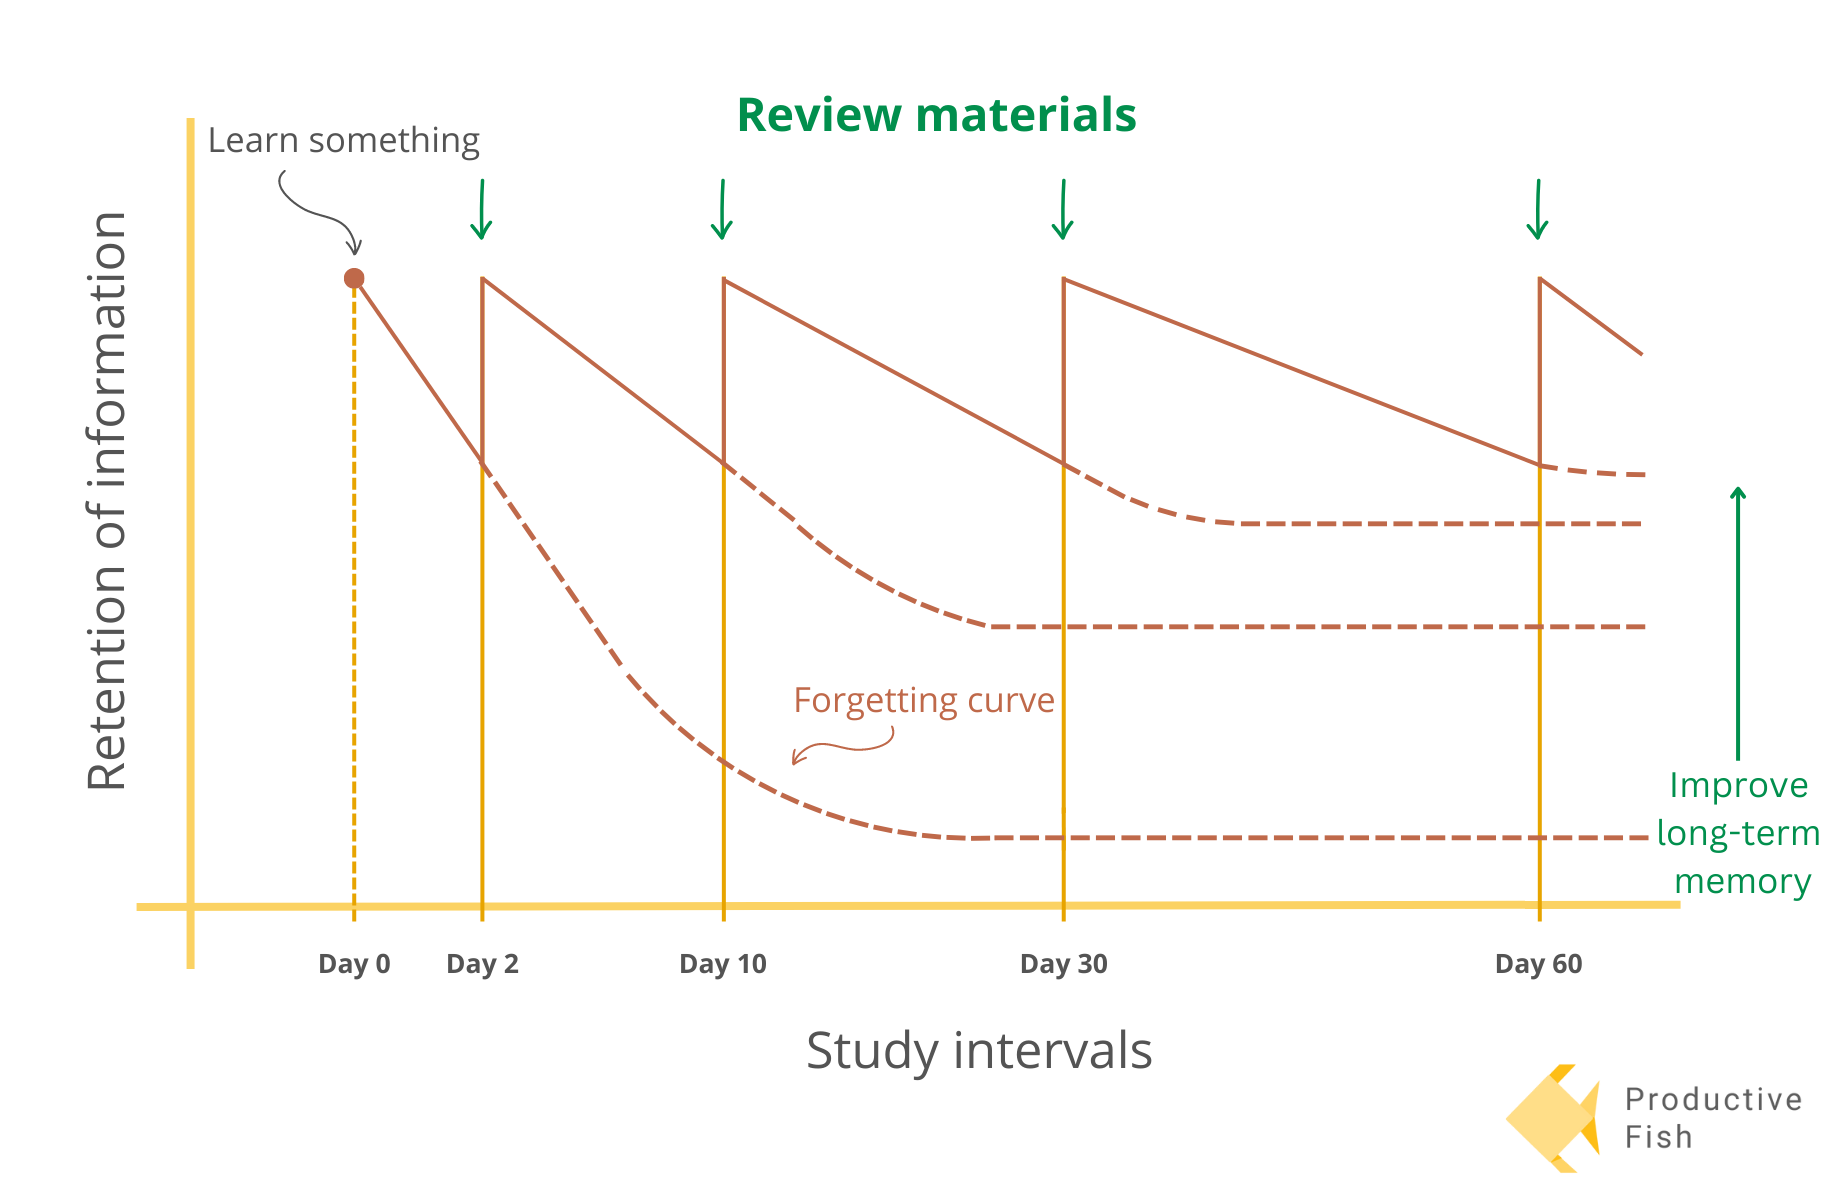
\includegraphics[width=\linewidth]{figures/spaced_repetition.png}
\caption{Spaced repetition: Memory declines over time, but a learner is more likely to remember something if they review it across multiple days
(\url{https://commons.wikimedia.org/wiki/File:Forgetting_curve_and_work_of_Ebbinghaus.png}, uploaded and dedicated to the universal public domain by user Productive.Fish).}
\end{figure}



%Now it’s not used to translate the web; but exercise are still based in translation (in both directions)
%(Interestingly, translation is otherwise not in vogue for in-class L2 learning!, more focused on like personal narratives and stuff)





\subsection{Evaluating Duolingo}

Like any popular product, Duolingo has critics as well as devoted fans.  Critics of Duolingo would note that it can only get learners to an Advanced Beginner or Low Intermediate ACTFL level (``able to handle
successfully a limited number of uncomplicated communicative tasks by
creating with the language in straightforward social situations'').
Courses on less-resourced languages are shorter and must promise an
even lower proficiency level.  Learners may find it frustrating for a
translation to be marked as wrong when the gist is correct or when
only one word is mis-typed.  Moreover, translating pre-written
sentences on Duolingo is arguably not as useful as learning to make
oneself understood in a spontaneous conversation.  According to \exword{Forbes}\footnote{``Game of tongues: How
Duolingo built a \$700 million business with its addictive
language-learning app,'' 16 July 2019, by Susan Adams, \exword{Forbes}.}, the Chief Revenue Officer of
Duolingo could not respond to the spoken question
\text{?`}\exword{Hablas espa\~nol?} `Do you speak Spanish?' after
six months of Duolingo Spanish.

Finally, like many other online courses, Duolingo struggles with
attrition.  Exact numbers are elusive and depend on the length of the
course, but course completion rates fall far below one percent.  (After 1277
consecutive days of studying Spanish, one of the authors of this
textbook is working through ``Intermediate Spanish, part 1,'' so
completing a course requires an extremely sustained commitment).

On the other hand, fans of Duolingo would argue that Duolingo is
better than nothing and teaches as much as can be expected in one or
two five-minute lessons per day.  The app is user-friendly, fun, and
always improving as researchers analyze data from millions of users.
Spontaneous production is the hardest, but Duolingo certainly improves
passive spoken and written comprehension and can serve as a valuable
complement or stepping stone to other exposure through schooling,
work, travel, socializing, or consuming media (including Duolingo's
own associated podcast) in the L2.  Through Duolingo for Schools,
teachers can assign Duolingo exercises as homework and track their
students' progress.  But should language teachers be grateful for
Duolingo as a supplementary tool, or should they feel threatened that
it may replace them?  This question -- about whether humans and
language technologies compete or complement one another -- will keep
coming back.

\section{Evaluation}

%\wdm{Pick up the Duolingo-specific last subsection and generalize it, explaining the need to evaluate learning outcomes, improve the system design and feedback to research. Mention randomized controlled field trials and A/B testing.} - tried to do this. -LG
Stepping back to CALL systems as a whole, how good are they? 
 They are surely better than nothing, but how do they compare to a traditional classroom? 
Taking inspiration from the still timely discussion of
\citet{Meskill:2002}, such systems have advantages and
disadvantages compared to in-person instruction.  Looking
first at the advantages, CALL tools can provide self-paced,
dynamically sequenced, automatically graded exercises to any number of
students across regions and time zones at scale, making L2 learning
accessible.  CALL tools can judge predetermined right-or-wrong answers
and provide immediate feedback in the form of
pre-written hints or corrections matched to the student's input.  Such
tools can record detailed information about the learner's progress,
providing data to both learners and researchers of L2 learning and
allowing for learner modeling and dynamic sequencing.  CALL tools can
provide authentic multimedia language usage and can motivate the
student's persistence through encouraging canned text, push
notifications, integration with ``likes'' on social media, and other
digital rewards.

As for the disadvantages, CALL tools still struggle to evaluate unexpected
input.  In an in-person introductory language class, students
learn to introduce themselves and to describe their own biography and
opinions, but such exercises are harder to automate in a CALL
system because there is no single correct answer.  CALL tools
therefore do not offer as many opportunities for a learner to practice
producing language extemporaneously.  Finally, the social element of
language learning is missing: The learner cannot engage in the process
-- arguably the end goal of L2 learning -- of trying to make
themselves understood in a real-life conversation.

To give learners greater opportunities for extemporaneous production, some language instructors have leveraged the dialog capabilities (discussed in \chapref{ch:dialog-systems}) of generative language models so that students can practice open-ended conversation in the target language, via speech or writing.  The dialog system could in principle be prompted to adjust its output to the student's L2 level.  Dialog systems allow the student to practice producing language at any time and frequency, without the logistical challenges or potential social anxiety of a human interlocutor.  But dialog systems do not currently grade the student's output for correctness, so they cannot model the learner's strengths and weaknesses as more structured CALL systems can.  It remains an open question how dialog systems will be integrated with other CALL tools.


The more people who use a CALL system, the more its designers can use large-scale usage data to improve.   User-experience researchers use \keyword{A/B
testing}, an experiment where learners are assigned randomly to one of
two conditions (A or B) which are compared with respect to some
outcome variable (for example, probability of passing a certain test,
number of minutes spent learning, probability of continuing or giving
up, and so on) that the researcher wants to maximize.  One condition
serves as the control group, where the system is kept as-is, while the
other condition pilots a new feature.  If the people who encounter the
new feature have a better outcome, the feature might be deemed
successful and implemented for all learners.  A/B testing is a type of
\keyword{between-subjects experiment}, meaning that the experiment
compares the outcome across different groups of people, each assigned
to a different condition.  Between-subjects experiments contrast with
\keyword{within-subjects experiments}, where the same person
encounters multiple different conditions at different times.  A/B
testing is used widely beyond CALL, in any context where a company
wants to use evidence to decide whether a new feature would improve
users' experience, but in a CALL context it could be used to choose
the exact exercises and feedback that are most instructive or
motivating.

In a similar spirit, education researchers might conduct a \keyword{randomized controlled field trial}.  Here, students -- or entire classrooms -- are randomly assigned to one teaching method or another.  For example, perhaps one classroom uses CALL tools as additional homework, while the other classroom does not; or perhaps some students are given a simpler CALL system, while others get a fancier version.  Then  researchers might test whether the two groups differ meaningfully in their performance on a year-end exam.   The students or classrooms must be assigned randomly to each condition, to control for confounding variables such as the students' starting level, socioeconomic status, and so on; that way, any difference that is found can be attributed to the intervention (the instruction method) rather than underlying differences between the learners.  (A careful researcher will also gather data on such variables to make sure that they are controlled across the randomized groups.) The trial will also be more robust if it includes many students or many classrooms, so that the results are not skewed by, for example, one classroom having a particularly good teacher.

Such trials take inspiration from medicine, where it is common to  assign patients randomly to take a drug or a placebo to then test whether the drug-taking patients heal faster or live longer than the placebo group (in a randomized controlled clinical trial).  The phrase \exword{field trial} indicates that the trial takes place in a real-world setting such as a classroom, rather than a clinical medical setting such as a hospital.  A/B testing is a type of randomized (field) trial because users are randomly assigned to one condition or the other, and then compared with respect to some outcome.  The phrase \exword{A/B testing} tends to be used more often in a corporate context, while \exword{randomized trials} are discussed by academics, but they are essentially the same idea -- using data to quantify the effectiveness of different teaching strategies.

Across both in-person learning and CALL tools, one of the biggest
challenges in L2 instruction is motivating the learners to continue
learning.  Therefore, designers of CALL tools focus on creating a
friendly \keyword{user experience}.  Error-correction messages are
written to be encouraging as well as metalinguistically illuminating; push notifications are piloted via A/B
testing to find the one most likely to get the learner to open a CALL
app; learners are modeled and exercises are sequenced to optimize
perseverance.  Example sentences are designed to be socially inclusive
and appropriate for children, and might describe interesting characters,
stories, or cultural knowledge to keep learners engaged.

In sum, designing a good CALL system requires insight from many
different areas, including the study of how people learn and what
motivates them (drawing on education, psychology, and behavioral
economics) as well as human-computer interaction, applied linguistics,
and language technology.

\section{Consequences}

By exploring all the things you learn when you learn a new language,
we hope to illuminate the richness of language both in its own right
and as a domain to be tackled computationally.  We might suggest
reading this chapter in tandem with \chapref{ch:mt} on machine
translation to compare what it means, for a human versus a computer,
to be multilingual. As machine translation improves, do you think
humans have less incentive to learn a new language?

Computer-assisted language learning also evokes larger debates in
education technology more generally.  On the one hand, web platforms
have made education more accessible than ever.  Whatever you want to
learn, you can most likely find a helpful video tutorial about it.
There are platforms that teach programming languages and music using
the same principles that underlie CALL,
offering progressively difficult bite-sized exercises in the learner's
zone of proximal development to be checked for objective correctness.
These tools are cheap and can be accessed by millions of people around
the world.

On the other hand, online learners often give up, and the people who
learn online most successfully are often those who were already highly
motivated and self-sufficient at the outset.  It remains difficult to
retain learners who have less commitment or confidence.  Moreover, to
the extent that education provides socialization as well as
information transmission, that element is diluted online.

Education technology took on new significance when some schools were closed
during the coronavirus pandemic.  Some students adapted to online
learning, but others suffered tragically.  What tools could have
helped those students, and what tools can help them improve now?  As
education evolves, to what extent should education technology be seen
as a complement or a competitor to in-person schooling?  Moreover, as artificial tools get better at integrating language with the larger visual and social context, will robots ever take over the role of in-person language teachers?

Each form of education has distinct pros and cons.  Whereas a single
teacher may struggle to teach multiple levels at once, education
technology can offer self-paced exercises customized to the zone of
proximal development of each learner.  And while a generalist teacher
may not know every topic deeply, high-budget educational technology
tools can leverage the knowledge of specialized content experts as
well as the insights from large-scale A/B testing.  In contrast,
online learning can be notoriously isolating and depressing, while an
in-person classroom can offer a socio-intellectual community where
students can feel welcome, motivated, connected, and understood
through person-to-person conversations.  It remains an open question
how the pros and cons of education technology should be balanced with
those of in-person schooling.


% education technology in general
% learner modeling, adaptive testing, etc, self paced, also Codecademy is another example of this.... bite sized exercises, spaced repetition
% education more available than ever before?
% but also, how to get people to actually take advantage of it? lot of people give up actually.
% to what extent is education actually social? this is a big question coming out of covid.....

% cool the end, do that.

% do we talk about POS tagging somewhere???
% lifting
% learner strategies
% construct under-representation.... 

\begin{tblsfilledsymbol}{Checklist}{test}

\begin{itemize}
\item Compare and contrast L1 and L2 learning.
\item Discuss metrics for measuring L2 success, and whether such metrics are  applicable to L1 learning.
\item Identify the factors that contribute to success in L2 learning.
\item Explain why learning is advanced by input pitched to one's zone of proximal development.
\item Explain the idea of spaced repetition and how it is used in Duolingo.
\item Give examples of the types of questions used by language tutoring systems.
\item Give examples of ways that a tutoring system can use learner modeling to teach more effectively.
\item Compare and contrast the capabilities of intelligent CALL systems versus dialog systems for L2 learning.
\item Discuss the pros and cons of Duolingo and explain whether you see it as a supplement or a threat to L2 learning in a classroom.
\item Discuss the affordances and limitations of practicing an L2 by conversing with a dialog system.
\item Give examples of A/B testing and why it might be useful in education as well as business.
\end{itemize}

\end{tblsfilledsymbol}


\begin{tblsfilledsymbol}{Exercises}{pencil}

\begin{enumerate}
\setcounter{enumi}{0}

\item  Search online to find videos from ACTFL at each proficiency level.  Can a partner correctly guess a speaker's ACTFL level from a video that you play them?

\item   Explore \url{www.wordbank.stanford.edu}\footnote{Accessed 2024-04-26.} for data and visualizations of the words that children learn at various ages around the world.  Can you find an example of a word that is learned much earlier in one language/culture than another? (Can you propose an explanation?)  What factors are predictive of a child's productive vocabulary size (the number of unique words that they produce) at each age?  

\item  A friend comes to you with a business idea: They want to make a Duolingo-like app to help babies learn their L1.  Do you think there is a market for such an app?  How would it compare or contrast to tutoring systems designed for an L2?


\item  Read online about some of Duolingo's competitors, Babbel and Rosetta Stone.  What are the pros and cons of each compared to Duolingo?

\item Choose a grammatical construction of English that L2 learners might struggle to learn (talk to a linguistics student for ideas!).  Write a multiple-choice question with plausible distractor items to test this construction.  Ask a friend or classmate to answer the question and offer feedback.

\end{enumerate}
\end{tblsfilledsymbol}


\begin{tblsfilledsymbol}{Futher reading}{book}


A general overview of the use of NLP in the context of language
learning is provided in \citet{Meurers-20}. A detailed discussion of
ICALL projects, including a historical overview and a characterization
of the techniques used, can be found in \citet{Heift.Schulze-07}.  

\citet{Munday:2016} describes Duolingo and argues that is a useful complement to classroom instruction.

\citet{Huang-etal:2022} review the literature about dialog systems for language learning.

On tutoring systems more generally, some classic references include \citet{Swartz.Yazdani-92} and \citet{Holland.Kaplan.Sams-2013}, as well as  \citet{Heift:2010} and \citet{Amaral.Meurers-11}  for language in particular. 

\end{tblsfilledsymbol}


